\chapter{Magnetisme}
\fancyfoot[LO,RE]{Fisika: Elektrisiteit en Magnetisme}
    

\label{m37830}
    \section{Inleiding}

\begin{minipage}{.5\textwidth}

Magnetisme is 'n krag wat sekere voorwerpe, genoem ``magnetiese'' voorwerpe, op mekaar kan uitoefen sonder om fisies aan mekaar te raak. 'n Magnetiese voorwerp is omring deur 'n ``magneetveld'' wat swakker word verder weg van die voorwerp. 'n Tweede voorwerp kan die magnetiese krag voel van die eerste voorwerp want dit voel die magneetveld.

\chapterstartvideo{VPfkk} 

Mense weet al duisende jare van magnetisme. Byvoorbeeld, \textsl{magneetsteen} is 'n magnetiese vorm van die ysteroksied mineraal \textsl{magnetiet}. Dit het die eienskap dat dit yster voorwerpe aantrek. Dit word in ou Europese en Asiese rekords genoem; vanaf rondom 800 \textsc{vC} in Europa en rondom 2~600 \textsc{vC} in Asi\"e. \par


\end{minipage}
\begin{minipage}{.5\textwidth}
\begin{center}
\textbf{Magnetiese voorwerpe sit vas aan 'n magneet.}\par
 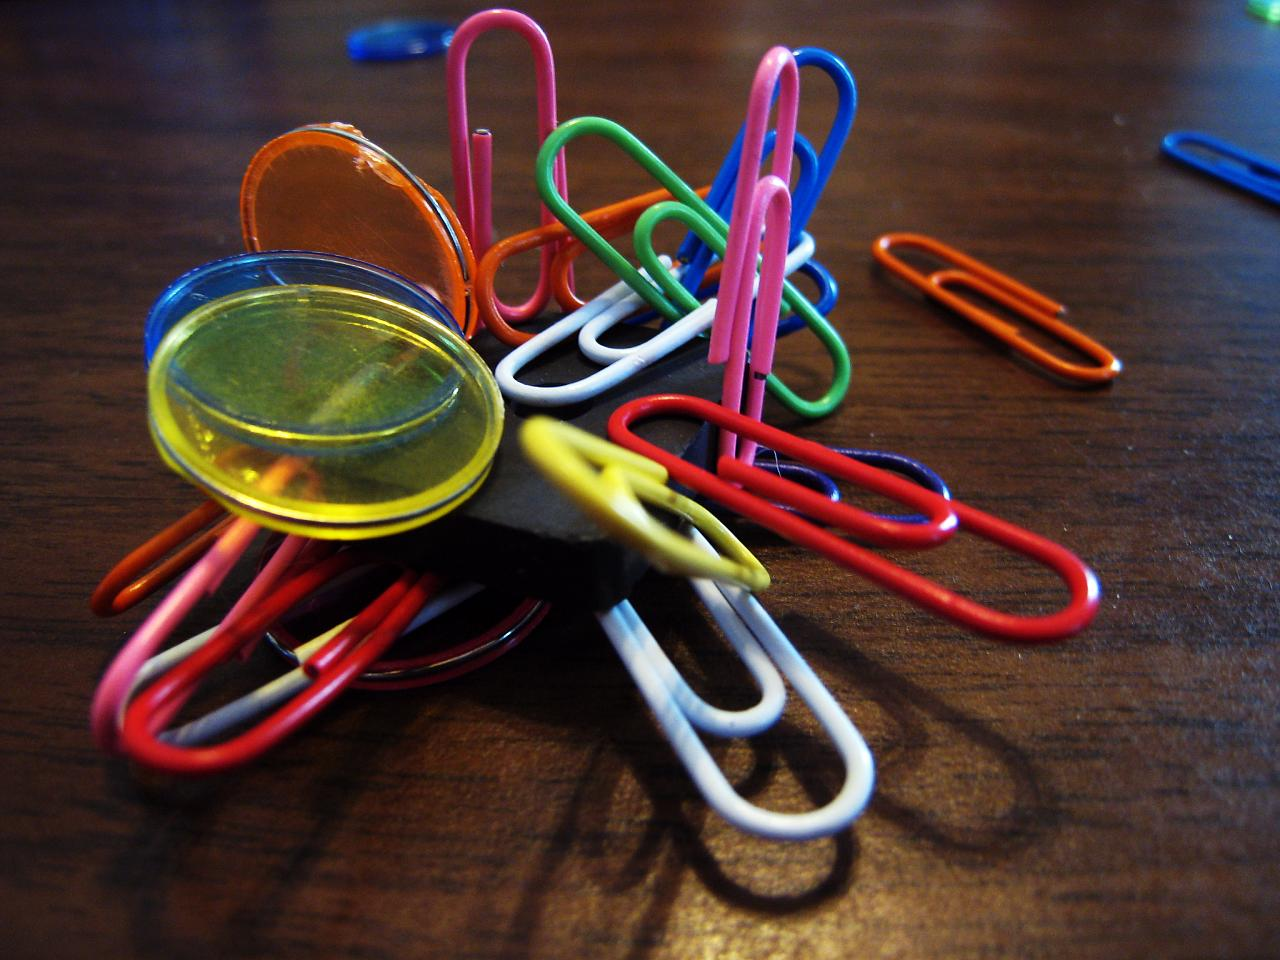
\includegraphics[width=.8\textwidth]{photos/magnet_mess_dougww.jpg}\par
\textit{Foto deur dougww op Flickr}
\end{center}
\end{minipage}
 
\IFact{Die woord \textsl{magneet} kom van die Griekse woord \textsl{magnes}, waarskynlik  van Magnesi\"e in Klein-Asi\"e, voorheen 'n belangrike bron van magneetsteen.}



\section*{Magnetiese velde}


 'n Magneetveld is die ruimte waar 'n magneet of voorwerp gemaak van magnetiese stof 'n krag sal ondervind sonder enige aanraking. \par

Elektrone binne enige voorwerp het magneetvelde wat met hulle geassosieer word. In die meeste stowwe is die rigting van hierdie velde in alle rigtings so die netto magneetveld is nul. Byvoorbeeld, in die plastiese bal hieronder wys die magneetvelde van die elektrone (aangedui met pyltjies) in alle rigtings en kanseleer mekaar uit. Die plastiekbal is dus nie magneties nie en het nie 'n magneetveld nie.

 
      \label{m37830*id128346}
    \setcounter{subfigure}{0}
	\begin{figure}[H] % horizontal\label{m37830*id128349}
    \begin{center}
  \begin{pspicture}(0,-1.5089062)(11.060625,1.4689063)
\pscircle[linewidth=0.04,dimen=outer](3.663125,0.45890626){1.01}
\psline[linewidth=0.04cm,arrowsize=0.05291667cm 2.0,arrowlength=1.4,arrowinset=0.4]{->}(4.013125,0.98890626)(4.173125,1.2489063)
\psline[linewidth=0.04cm,arrowsize=0.05291667cm 2.0,arrowlength=1.4,arrowinset=0.4]{->}(2.933125,0.12890625)(3.213125,0.04890625)
\psline[linewidth=0.04cm,arrowsize=0.05291667cm 2.0,arrowlength=1.4,arrowinset=0.4]{->}(3.693125,-0.45109376)(3.633125,-0.19109374)
\psline[linewidth=0.04cm,arrowsize=0.05291667cm 2.0,arrowlength=1.4,arrowinset=0.4]{->}(3.933125,-0.07109375)(3.753125,-0.27109376)
\psline[linewidth=0.04cm,arrowsize=0.05291667cm 2.0,arrowlength=1.4,arrowinset=0.4]{->}(3.793125,-0.27109376)(4.113125,-0.33109376)
\psline[linewidth=0.04cm,arrowsize=0.05291667cm 2.0,arrowlength=1.4,arrowinset=0.4]{->}(3.133125,0.9089062)(3.413125,0.82890624)
\psline[linewidth=0.04cm,arrowsize=0.05291667cm 2.0,arrowlength=1.4,arrowinset=0.4]{->}(4.053125,0.22890624)(4.333125,0.14890625)
\psline[linewidth=0.04cm,arrowsize=0.05291667cm 2.0,arrowlength=1.4,arrowinset=0.4]{->}(2.833125,0.22890624)(2.993125,0.48890626)
\psline[linewidth=0.04cm,arrowsize=0.05291667cm 2.0,arrowlength=1.4,arrowinset=0.4]{->}(2.973125,0.60890627)(3.253125,0.5289062)
\psline[linewidth=0.04cm,arrowsize=0.05291667cm 2.0,arrowlength=1.4,arrowinset=0.4]{->}(2.833125,0.22890624)(2.993125,0.48890626)
\psline[linewidth=0.04cm,arrowsize=0.05291667cm 2.0,arrowlength=1.4,arrowinset=0.4]{->}(2.913125,0.70890623)(3.073125,0.9689062)
\psline[linewidth=0.04cm,arrowsize=0.05291667cm 2.0,arrowlength=1.4,arrowinset=0.4]{->}(2.913125,0.70890623)(3.073125,0.9689062)
\psline[linewidth=0.04cm,arrowsize=0.05291667cm 2.0,arrowlength=1.4,arrowinset=0.4]{->}(3.233125,-0.17109375)(3.393125,0.08890625)
\psline[linewidth=0.04cm,arrowsize=0.05291667cm 2.0,arrowlength=1.4,arrowinset=0.4]{->}(3.293125,0.26890624)(3.453125,0.5289062)
\psline[linewidth=0.04cm,arrowsize=0.05291667cm 2.0,arrowlength=1.4,arrowinset=0.4]{->}(3.313125,1.0289062)(3.473125,1.2889062)
\psline[linewidth=0.04cm,arrowsize=0.05291667cm 2.0,arrowlength=1.4,arrowinset=0.4]{->}(3.313125,1.0289062)(3.473125,1.2889062)
\psline[linewidth=0.04cm,arrowsize=0.05291667cm 2.0,arrowlength=1.4,arrowinset=0.4]{->}(3.513125,0.82890624)(3.673125,1.0889063)
\psline[linewidth=0.04cm,arrowsize=0.05291667cm 2.0,arrowlength=1.4,arrowinset=0.4]{->}(4.213125,0.7889063)(4.373125,1.0489062)
\psline[linewidth=0.04cm,arrowsize=0.05291667cm 2.0,arrowlength=1.4,arrowinset=0.4]{->}(4.073125,-0.19109374)(4.233125,0.06890625)
\psline[linewidth=0.04cm,arrowsize=0.05291667cm 2.0,arrowlength=1.4,arrowinset=0.4]{->}(4.553125,0.30890626)(4.273125,0.42890626)
\psline[linewidth=0.04cm,arrowsize=0.05291667cm 2.0,arrowlength=1.4,arrowinset=0.4]{->}(3.973125,0.74890625)(3.693125,0.86890626)
\psline[linewidth=0.04cm,arrowsize=0.05291667cm 2.0,arrowlength=1.4,arrowinset=0.4]{->}(3.673125,0.02890625)(3.393125,0.14890625)
\psline[linewidth=0.04cm,arrowsize=0.05291667cm 2.0,arrowlength=1.4,arrowinset=0.4]{->}(3.513125,0.60890627)(3.233125,0.7289063)
\psline[linewidth=0.04cm,arrowsize=0.05291667cm 2.0,arrowlength=1.4,arrowinset=0.4]{->}(3.493125,-0.35109374)(3.213125,-0.23109375)
\psline[linewidth=0.04cm,arrowsize=0.05291667cm 2.0,arrowlength=1.4,arrowinset=0.4]{->}(3.293125,0.18890625)(3.013125,0.30890626)
\psline[linewidth=0.04cm,arrowsize=0.05291667cm 2.0,arrowlength=1.4,arrowinset=0.4]{->}(3.893125,0.06890625)(3.893125,0.34890625)
\psline[linewidth=0.04cm,arrowsize=0.05291667cm 2.0,arrowlength=1.4,arrowinset=0.4]{->}(3.653125,0.5289062)(3.653125,0.80890626)
\psline[linewidth=0.04cm,arrowsize=0.05291667cm 2.0,arrowlength=1.4,arrowinset=0.4]{->}(3.553125,0.20890625)(3.553125,0.48890626)
\psline[linewidth=0.04cm,arrowsize=0.05291667cm 2.0,arrowlength=1.4,arrowinset=0.4]{->}(3.453125,-0.25109375)(3.453125,0.02890625)
\psline[linewidth=0.04cm,arrowsize=0.05291667cm 2.0,arrowlength=1.4,arrowinset=0.4]{->}(3.173125,0.9689062)(3.173125,1.2489063)
\psline[linewidth=0.04cm,arrowsize=0.05291667cm 2.0,arrowlength=1.4,arrowinset=0.4]{->}(4.473125,0.82890624)(4.473125,0.48890626)
\psline[linewidth=0.04cm,arrowsize=0.05291667cm 2.0,arrowlength=1.4,arrowinset=0.4]{->}(3.733125,0.50890625)(3.733125,0.16890626)
\psline[linewidth=0.04cm,arrowsize=0.05291667cm 2.0,arrowlength=1.4,arrowinset=0.4]{->}(3.933125,0.30890626)(4.073125,0.5889062)
\psline[linewidth=0.04cm,arrowsize=0.05291667cm 2.0,arrowlength=1.4,arrowinset=0.4]{->}(4.013125,0.92890626)(4.013125,0.5889062)
\psline[linewidth=0.04cm,arrowsize=0.05291667cm 2.0,arrowlength=1.4,arrowinset=0.4]{->}(4.213125,0.7289063)(4.213125,0.38890624)
\psline[linewidth=0.04cm,arrowsize=0.05291667cm 2.0,arrowlength=1.4,arrowinset=0.4]{->}(3.073125,0.02890625)(3.073125,-0.31109375)
\psline[linewidth=0.04cm,arrowsize=0.05291667cm 2.0,arrowlength=1.4,arrowinset=0.4]{->}(4.313125,0.14890625)(4.313125,-0.19109374)
\psline[linewidth=0.04cm,arrowsize=0.05291667cm 2.0,arrowlength=1.4,arrowinset=0.4]{->}(3.933125,1.2089063)(3.653125,1.3289063)
\psline[linewidth=0.04cm,arrowsize=0.05291667cm 2.0,arrowlength=1.4,arrowinset=0.4]{->}(3.693125,1.0689063)(3.973125,0.98890626)
\psline[linewidth=0.04cm](4.293125,0.9689062)(5.393125,1.1689062)
\psline[linewidth=0.04cm](4.453125,0.6689063)(5.373125,1.1689062)
\psline[linewidth=0.04cm](5.373125,1.1689062)(5.713125,1.1689062)
\psline[linewidth=0.04cm](4.613125,0.18890625)(5.733125,0.18890625)
\rput(6.89,0.19890624){plastiese bal}
\rput(9.090938,1.1789062){rigtings van elektrone se magneet velde}
\rput(3.9001563,-0.86109376){Die elektrone se magneetvelde wys in alle rigtings}
\rput(3.7371874,-1.2810937){dus is daar nie 'n netto magneetveld vir die hele bal nie.}
\end{pspicture} 
  \end{center}
 \end{figure}       
      \par 

In sommige stowwe (bv. yster), die \textbf{ferromagnetiese} stowwe, is daar gebiede genoem die \textsl{domein}, waar die elektrone se magneetvelde in lyn met mekaar gebring word. Al die atome in elke domein is gegroepeer sodat die magneetvelde van hulle elektrone in dieselfde rigting wys. Die diagram wys 'n stuk van 'n ysternaald, ingezoom om die domeine  te wys, met die magneetvelde wat in een rigting gerig is.



\begin{figure}[H] % horizontal\label{m37830*id128374}
\begin{center}
\begin{pspicture}(0,-2.5045311)(10.473125,2.4845312)
\definecolor{color3b}{rgb}{0.8,0.8,0.8}
\psframe[linewidth=0.04,dimen=outer,fillstyle=solid,fillcolor=color3b](6.36,0.50453126)(1.08,-0.83546877)
\psbezier[linewidth=0.04,fillstyle=solid,fillcolor=color3b](0.0,2.1345313)(0.0,2.0820312)(7.4,1.7445313)(7.46,2.1045313)(7.52,2.4645312)(0.0,2.1870313)(0.0,2.1345313)
\psellipse[linewidth=0.04,dimen=outer,fillstyle=solid](6.8,2.1045313)(0.26,0.1)
\psline[linewidth=0.04cm](3.06,2.2845314)(3.06,1.9845313)
\psline[linewidth=0.04cm](4.04,2.2845314)(4.04,1.9245312)
\psline[linewidth=0.04cm,linestyle=dashed,dash=0.16cm 0.16cm](3.06,1.9845313)(1.12,0.48453125)
\psline[linewidth=0.04cm,linestyle=dashed,dash=0.16cm 0.16cm](4.02,1.9445312)(6.34,0.50453126)
\psbezier[linewidth=0.04](1.12,-0.11546875)(1.12,-0.91546875)(2.16,0.16453125)(2.34,0.18453126)(2.52,0.20453125)(2.88,-0.29546875)(2.88,0.50453126)
\psbezier[linewidth=0.04](2.06,0.02453125)(2.34,-0.47546875)(3.42,-0.39546874)(3.26,-0.79546875)
\psbezier[linewidth=0.04](3.28,-0.8154687)(3.32,0.52453125)(4.02,-0.27546874)(4.52,-0.21546875)(5.02,-0.15546875)(5.58,-0.37546876)(5.58,0.48453125)
\psbezier[linewidth=0.04](3.42,-0.13546875)(3.56,0.10453125)(4.08,0.12453125)(3.98,0.50453126)
\psbezier[linewidth=0.04](5.34,-0.09546875)(5.34,-0.39546874)(6.34,-0.5154688)(6.34,-0.21546875)
\psbezier[linewidth=0.04](5.34,-0.11546875)(5.38,-0.33546874)(5.96,-0.33546874)(5.22,-0.79546875)
\psline[linewidth=0.04cm,arrowsize=0.05291667cm 2.0,arrowlength=1.4,arrowinset=0.4]{->}(1.16,0.12453125)(1.38,0.44453126)
\psline[linewidth=0.04cm,arrowsize=0.05291667cm 2.0,arrowlength=1.4,arrowinset=0.4]{->}(1.2,-0.15546875)(1.42,0.16453125)
\psline[linewidth=0.04cm,arrowsize=0.05291667cm 2.0,arrowlength=1.4,arrowinset=0.4]{->}(1.46,0.10453125)(1.68,0.42453125)
\psline[linewidth=0.04cm,arrowsize=0.05291667cm 2.0,arrowlength=1.4,arrowinset=0.4]{->}(1.26,-0.35546875)(1.48,-0.03546875)
\psline[linewidth=0.04cm,arrowsize=0.05291667cm 2.0,arrowlength=1.4,arrowinset=0.4]{->}(1.58,-0.19546875)(1.8,0.12453125)
\psline[linewidth=0.04cm,arrowsize=0.05291667cm 2.0,arrowlength=1.4,arrowinset=0.4]{->}(1.64,0.10453125)(1.86,0.42453125)
\psline[linewidth=0.04cm,arrowsize=0.05291667cm 2.0,arrowlength=1.4,arrowinset=0.4]{->}(1.86,0.04453125)(2.08,0.36453125)
\psline[linewidth=0.04cm,arrowsize=0.05291667cm 2.0,arrowlength=1.4,arrowinset=0.4]{->}(2.16,0.14453125)(2.38,0.46453124)
\psline[linewidth=0.04cm,arrowsize=0.05291667cm 2.0,arrowlength=1.4,arrowinset=0.4]{->}(2.62,0.14453125)(2.84,0.46453124)
\psline[linewidth=0.04cm,arrowsize=0.05291667cm 2.0,arrowlength=1.4,arrowinset=0.4]{->}(2.42,0.20453125)(2.64,0.52453125)
\psline[linewidth=0.04cm,arrowsize=0.05291667cm 2.0,arrowlength=1.4,arrowinset=0.4]{->}(1.2,-0.7554687)(1.2,-0.39546874)
\psline[linewidth=0.04cm,arrowsize=0.05291667cm 2.0,arrowlength=1.4,arrowinset=0.4]{->}(1.38,-0.77546877)(1.38,-0.41546875)
\psline[linewidth=0.04cm,arrowsize=0.05291667cm 2.0,arrowlength=1.4,arrowinset=0.4]{->}(1.54,-0.73546875)(1.54,-0.37546876)
\psline[linewidth=0.04cm,arrowsize=0.05291667cm 2.0,arrowlength=1.4,arrowinset=0.4]{->}(1.72,-0.79546875)(1.72,-0.43546876)
\psline[linewidth=0.04cm,arrowsize=0.05291667cm 2.0,arrowlength=1.4,arrowinset=0.4]{->}(1.86,-0.5754688)(1.86,-0.21546875)
\psline[linewidth=0.04cm,arrowsize=0.05291667cm 2.0,arrowlength=1.4,arrowinset=0.4]{->}(1.96,-0.77546877)(1.96,-0.41546875)
\psline[linewidth=0.04cm,arrowsize=0.05291667cm 2.0,arrowlength=1.4,arrowinset=0.4]{->}(2.04,-0.43546876)(2.04,-0.07546875)
\psline[linewidth=0.04cm,arrowsize=0.05291667cm 2.0,arrowlength=1.4,arrowinset=0.4]{->}(2.76,-0.73546875)(2.76,-0.37546876)
\psline[linewidth=0.04cm,arrowsize=0.05291667cm 2.0,arrowlength=1.4,arrowinset=0.4]{->}(2.54,-0.67546874)(2.54,-0.31546876)
\psline[linewidth=0.04cm,arrowsize=0.05291667cm 2.0,arrowlength=1.4,arrowinset=0.4]{->}(2.36,-0.79546875)(2.36,-0.43546876)
\psline[linewidth=0.04cm,arrowsize=0.05291667cm 2.0,arrowlength=1.4,arrowinset=0.4]{->}(2.16,-0.6354687)(2.16,-0.27546874)
\psline[linewidth=0.04cm,arrowsize=0.05291667cm 2.0,arrowlength=1.4,arrowinset=0.4]{->}(3.34,-0.6954687)(3.76,-0.6954687)
\psline[linewidth=0.04cm,arrowsize=0.05291667cm 2.0,arrowlength=1.4,arrowinset=0.4]{->}(3.4,-0.53546876)(3.82,-0.53546876)
\psline[linewidth=0.04cm,arrowsize=0.05291667cm 2.0,arrowlength=1.4,arrowinset=0.4]{->}(3.4,-0.35546875)(3.82,-0.35546875)
\psline[linewidth=0.04cm,arrowsize=0.05291667cm 2.0,arrowlength=1.4,arrowinset=0.4]{->}(3.84,-0.6354687)(4.26,-0.6354687)
\psline[linewidth=0.04cm,arrowsize=0.05291667cm 2.0,arrowlength=1.4,arrowinset=0.4]{->}(3.92,-0.41546875)(4.34,-0.41546875)
\psline[linewidth=0.04cm,arrowsize=0.05291667cm 2.0,arrowlength=1.4,arrowinset=0.4]{->}(3.62,-0.21546875)(4.04,-0.21546875)
\psline[linewidth=0.04cm,arrowsize=0.05291667cm 2.0,arrowlength=1.4,arrowinset=0.4]{->}(4.28,-0.71546876)(4.7,-0.71546876)
\psline[linewidth=0.04cm,arrowsize=0.05291667cm 2.0,arrowlength=1.4,arrowinset=0.4]{->}(4.08,-0.5154688)(4.5,-0.5154688)
\psline[linewidth=0.04cm,arrowsize=0.05291667cm 2.0,arrowlength=1.4,arrowinset=0.4]{->}(4.32,-0.31546876)(4.74,-0.31546876)
\psline[linewidth=0.04cm,arrowsize=0.05291667cm 2.0,arrowlength=1.4,arrowinset=0.4]{->}(4.56,-0.55546874)(4.98,-0.55546874)
\psline[linewidth=0.04cm,arrowsize=0.05291667cm 2.0,arrowlength=1.4,arrowinset=0.4]{->}(4.74,-0.37546876)(5.16,-0.37546876)
\psline[linewidth=0.04cm,arrowsize=0.05291667cm 2.0,arrowlength=1.4,arrowinset=0.4]{->}(4.76,-0.67546874)(5.18,-0.67546874)
\psline[linewidth=0.04cm,arrowsize=0.05291667cm 2.0,arrowlength=1.4,arrowinset=0.4]{->}(5.02,-0.49546874)(5.44,-0.49546874)
\psline[linewidth=0.04cm,arrowsize=0.05291667cm 2.0,arrowlength=1.4,arrowinset=0.4]{->}(2.44,-0.17546874)(2.22,0.10453125)
\psline[linewidth=0.04cm,arrowsize=0.05291667cm 2.0,arrowlength=1.4,arrowinset=0.4]{->}(2.68,-0.23546875)(2.46,0.04453125)
\psline[linewidth=0.04cm,arrowsize=0.05291667cm 2.0,arrowlength=1.4,arrowinset=0.4]{->}(2.94,-0.37546876)(2.72,-0.09546875)
\psline[linewidth=0.04cm,arrowsize=0.05291667cm 2.0,arrowlength=1.4,arrowinset=0.4]{->}(3.24,-0.47546875)(3.02,-0.19546875)
\psline[linewidth=0.04cm,arrowsize=0.05291667cm 2.0,arrowlength=1.4,arrowinset=0.4]{->}(3.12,-0.19546875)(2.9,0.08453125)
\psline[linewidth=0.04cm,arrowsize=0.05291667cm 2.0,arrowlength=1.4,arrowinset=0.4]{->}(3.18,0.12453125)(2.96,0.40453124)
\psline[linewidth=0.04cm,arrowsize=0.05291667cm 2.0,arrowlength=1.4,arrowinset=0.4]{->}(3.28,-0.19546875)(3.06,0.08453125)
\psline[linewidth=0.04cm,arrowsize=0.05291667cm 2.0,arrowlength=1.4,arrowinset=0.4]{->}(3.42,0.04453125)(3.2,0.32453126)
\psline[linewidth=0.04cm,arrowsize=0.05291667cm 2.0,arrowlength=1.4,arrowinset=0.4]{->}(3.54,0.16453125)(3.32,0.44453126)
\psline[linewidth=0.04cm,arrowsize=0.05291667cm 2.0,arrowlength=1.4,arrowinset=0.4]{->}(3.72,0.16453125)(3.5,0.44453126)
\psline[linewidth=0.04cm,arrowsize=0.05291667cm 2.0,arrowlength=1.4,arrowinset=0.4]{->}(3.98,0.24453124)(4.0,-0.09546875)
\psline[linewidth=0.04cm,arrowsize=0.05291667cm 2.0,arrowlength=1.4,arrowinset=0.4]{->}(4.1,0.46453124)(4.12,0.12453125)
\psline[linewidth=0.04cm,arrowsize=0.05291667cm 2.0,arrowlength=1.4,arrowinset=0.4]{->}(4.22,0.22453125)(4.24,-0.11546875)
\psline[linewidth=0.04cm,arrowsize=0.05291667cm 2.0,arrowlength=1.4,arrowinset=0.4]{->}(4.36,0.42453125)(4.38,0.08453125)
\psline[linewidth=0.04cm,arrowsize=0.05291667cm 2.0,arrowlength=1.4,arrowinset=0.4]{->}(4.46,0.12453125)(4.48,-0.21546875)
\psline[linewidth=0.04cm,arrowsize=0.05291667cm 2.0,arrowlength=1.4,arrowinset=0.4]{->}(4.58,0.48453125)(4.6,0.14453125)
\psline[linewidth=0.04cm,arrowsize=0.05291667cm 2.0,arrowlength=1.4,arrowinset=0.4]{->}(4.7,0.22453125)(4.72,-0.11546875)
\psline[linewidth=0.04cm,arrowsize=0.05291667cm 2.0,arrowlength=1.4,arrowinset=0.4]{->}(4.86,0.32453126)(4.88,-0.01546875)
\psline[linewidth=0.04cm,arrowsize=0.05291667cm 2.0,arrowlength=1.4,arrowinset=0.4]{->}(5.0,0.42453125)(5.02,0.08453125)
\psline[linewidth=0.04cm,arrowsize=0.05291667cm 2.0,arrowlength=1.4,arrowinset=0.4]{->}(5.14,0.26453125)(5.16,-0.07546875)
\psline[linewidth=0.04cm,arrowsize=0.05291667cm 2.0,arrowlength=1.4,arrowinset=0.4]{->}(5.32,0.36453125)(5.34,0.02453125)
\psline[linewidth=0.04cm,arrowsize=0.05291667cm 2.0,arrowlength=1.4,arrowinset=0.4]{->}(5.8,-0.15546875)(5.42,-0.15546875)
\psline[linewidth=0.04cm,arrowsize=0.05291667cm 2.0,arrowlength=1.4,arrowinset=0.4]{->}(6.18,-0.29546875)(5.8,-0.29546875)
\psline[linewidth=0.04cm,arrowsize=0.05291667cm 2.0,arrowlength=1.4,arrowinset=0.4]{->}(6.16,-0.03546875)(5.78,-0.03546875)
\psline[linewidth=0.04cm,arrowsize=0.05291667cm 2.0,arrowlength=1.4,arrowinset=0.4]{->}(5.94,0.08453125)(5.56,0.08453125)
\psline[linewidth=0.04cm,arrowsize=0.05291667cm 2.0,arrowlength=1.4,arrowinset=0.4]{->}(6.22,0.22453125)(5.84,0.22453125)
\psline[linewidth=0.04cm,arrowsize=0.05291667cm 2.0,arrowlength=1.4,arrowinset=0.4]{->}(6.0,0.36453125)(5.62,0.36453125)
\psline[linewidth=0.04cm,arrowsize=0.05291667cm 2.0,arrowlength=1.4,arrowinset=0.4]{->}(5.7,-0.45546874)(5.46,-0.7554687)
\psline[linewidth=0.04cm,arrowsize=0.05291667cm 2.0,arrowlength=1.4,arrowinset=0.4]{->}(5.86,-0.47546875)(5.62,-0.77546877)
\psline[linewidth=0.04cm,arrowsize=0.05291667cm 2.0,arrowlength=1.4,arrowinset=0.4]{->}(6.3,-0.41546875)(6.06,-0.71546876)
\psline[linewidth=0.04cm,arrowsize=0.05291667cm 2.0,arrowlength=1.4,arrowinset=0.4]{->}(6.06,-0.49546874)(5.82,-0.79546875)
\psline[linewidth=0.103999995cm,linecolor=white,arrowsize=0.05291667cm 2.0,arrowlength=1.4,arrowinset=0.4]{->}(1.48,-0.13546875)(1.84,0.28453124)
\psline[linewidth=0.103999995cm,linecolor=white,arrowsize=0.05291667cm 2.0,arrowlength=1.4,arrowinset=0.4]{->}(2.041348,-0.6820518)(2.0386522,-0.1288857)
\psline[linewidth=0.103999995cm,linecolor=white,arrowsize=0.05291667cm 2.0,arrowlength=1.4,arrowinset=0.4]{->}(3.3071501,-0.1291224)(2.93285,0.27818492)
\psline[linewidth=0.103999995cm,linecolor=white,arrowsize=0.05291667cm 2.0,arrowlength=1.4,arrowinset=0.4]{->}(4.023517,-0.4179114)(4.5764832,-0.4330261)
\psline[linewidth=0.103999995cm,linecolor=white,arrowsize=0.05291667cm 2.0,arrowlength=1.4,arrowinset=0.4]{->}(4.760891,0.41111615)(4.759109,-0.14205365)
\psline[linewidth=0.103999995cm,linecolor=white,arrowsize=0.05291667cm 2.0,arrowlength=1.4,arrowinset=0.4]{->}(6.176575,0.052041616)(5.623425,0.057020884)
\psline[linewidth=0.103999995cm,linecolor=white,arrowsize=0.05291667cm 2.0,arrowlength=1.4,arrowinset=0.4]{->}(6.1610656,-0.41638675)(5.7989345,-0.83455074)
\psline[linewidth=0.04cm](7.12,1.9645313)(7.88,1.4445312)
\rput(8.651875,1.3995312){\footnotesize  yster naald}
\psline[linewidth=0.04cm](6.32,0.02453125)(7.32,0.02453125)
\rput(8.923282,0.05953125){\footnotesize ingezoomde deel van naald}
\psline[linewidth=0.04cm](2.18,-0.83546877)(3.36,-1.5554688)
\psline[linewidth=0.04cm](4.0,-0.8154687)(3.34,-1.5554688)
\rput(4.642031,-1.7804687){\footnotesize Die magneetvelde van die elektrone in elke domein (swart pyltjies)}
\rput(3.9789062,-2.0404687){\footnotesize wys in dieselfde rigting. Dit veroorsaak 'n netto}
\rput(4.067969,-2.3004687){\footnotesize magneet veld (groot wit pyle) in elke domein}
\end{pspicture} 
    \end{center}
 \end{figure}       

\par 
In permanente magnete is daar baie domeine wat gerig is, dus is daar 'n \textsl{netto magneetveld}. Voorwerpe wat van ferromagnetiese materiaal gemaak is kan gemagnetiseer word, bv. deur 'n magneet in een rigting te vryf teen die voorwerp. Dit veroorsaak dat die magneetvelde van meeste, indien nie al die domeine in een rigting gerig word. Die resultaat is dat die voorwerp as 'n geheel 'n netto magneetveld het. Dit is dan \textsl{magneties}. Sodra 'n ferromagnetiese voorwerp gemagnetiseerd is, sal dit magneties bly sonder 'n ander magneet in die nabyheid (D.w.s. sonder 'n eksterne magneetveld). Die diagram hieronder wys 'n naald wat gemagnetiseerd is, want die magneetvelde in elke domein wys in dieselde rigting. \par

\begin{minipage}{.3\textwidth}
\begin{center}
\textbf{ 'n Permanente magneet}\par
 \includegraphics[width=.8\textwidth]{photos/HarshPatelPhotographer.jpg}\par
\textit{Foto deur Harsh Patel}
\end{center}
\end{minipage}
\begin{minipage}{.7\textwidth}
      
      \label{m37830*id128400}
    \setcounter{subfigure}{0}
	\begin{figure}[H] % horizontal\label{m37830*id128403}
    \begin{center}
\begin{pspicture}(0,-2.5045311)(10.473125,2.4845312)
\definecolor{color3b}{rgb}{0.8,0.8,0.8}
\psframe[linewidth=0.04,dimen=outer,fillstyle=solid,fillcolor=color3b](6.36,0.50453126)(1.08,-0.83546877)
\psbezier[linewidth=0.04,fillstyle=solid,fillcolor=color3b](0.0,2.1345313)(0.0,2.0820312)(7.4,1.7445313)(7.46,2.1045313)(7.52,2.4645312)(0.0,2.1870313)(0.0,2.1345313)
\psellipse[linewidth=0.04,dimen=outer,fillstyle=solid](6.8,2.1045313)(0.26,0.1)
\psline[linewidth=0.04cm](3.06,2.2845314)(3.06,1.9845313)
\psline[linewidth=0.04cm](4.04,2.2845314)(4.04,1.9245312)
\psline[linewidth=0.04cm,linestyle=dashed,dash=0.16cm 0.16cm](3.06,1.9845313)(1.12,0.48453125)
\psline[linewidth=0.04cm,linestyle=dashed,dash=0.16cm 0.16cm](4.02,1.9445312)(6.34,0.50453126)
\psbezier[linewidth=0.04](1.12,-0.11546875)(1.12,-0.91546875)(2.16,0.16453125)(2.34,0.18453126)(2.52,0.20453125)(2.88,-0.29546875)(2.88,0.50453126)
\psbezier[linewidth=0.04](2.06,0.02453125)(2.34,-0.47546875)(3.42,-0.39546874)(3.26,-0.79546875)
\psbezier[linewidth=0.04](3.28,-0.8154687)(3.32,0.52453125)(4.02,-0.27546874)(4.52,-0.21546875)(5.02,-0.15546875)(5.58,-0.37546876)(5.58,0.48453125)
\psbezier[linewidth=0.04](3.42,-0.13546875)(3.56,0.10453125)(4.08,0.12453125)(3.98,0.50453126)
\psbezier[linewidth=0.04](5.34,-0.09546875)(5.34,-0.39546874)(6.34,-0.5154688)(6.34,-0.21546875)
\psbezier[linewidth=0.04](5.34,-0.11546875)(5.38,-0.33546874)(5.96,-0.33546874)(5.22,-0.79546875)
\psline[linewidth=0.103999995cm,linecolor=white,arrowsize=0.05291667cm 2.0,arrowlength=1.4,arrowinset=0.4]{->}(4.283559,0.12556379)(4.836441,0.1434987)
\psline[linewidth=0.04cm](7.12,1.9645313)(7.88,1.4445312)
\rput(8.651875,1.3995312){\footnotesize yster naald}
\psline[linewidth=0.04cm](6.32,0.02453125)(7.32,0.02453125)
\rput(8.923282,0.05953125){\footnotesize ingezoomde deel van naald}
\psline[linewidth=0.04cm](2.18,-0.83546877)(3.36,-1.5554688)
\psline[linewidth=0.04cm](4.0,-0.8154687)(3.34,-1.5554688)
\rput(4.145625,-1.7804687){\footnotesize wanneer die naald gemagnetiseerd is, wys die magneetvelde}
\rput(3.8645313,-2.0404687){\footnotesize van al die domeine (wit pyle) in dieselfde rigting }
\rput(3.7326562,-2.3004687){\footnotesize en veroorsaak dus 'n netto magneetveld}
\psline[linewidth=0.103999995cm,linecolor=white,arrowsize=0.05291667cm 2.0,arrowlength=1.4,arrowinset=0.4]{->}(4.123559,-0.4944362)(4.6764407,-0.4765013)
\psline[linewidth=0.103999995cm,linecolor=white,arrowsize=0.05291667cm 2.0,arrowlength=1.4,arrowinset=0.4]{->}(1.323559,0.16556379)(1.8764409,0.18349871)
\psline[linewidth=0.103999995cm,linecolor=white,arrowsize=0.05291667cm 2.0,arrowlength=1.4,arrowinset=0.4]{->}(2.7035592,-0.11443621)(3.2564409,-0.09650129)
\psline[linewidth=0.103999995cm,linecolor=white,arrowsize=0.05291667cm 2.0,arrowlength=1.4,arrowinset=0.4]{->}(1.6435591,-0.5544362)(2.196441,-0.5365013)
\psline[linewidth=0.103999995cm,linecolor=white,arrowsize=0.05291667cm 2.0,arrowlength=1.4,arrowinset=0.4]{->}(5.663559,0.085563794)(6.216441,0.103498705)
\psline[linewidth=0.103999995cm,linecolor=white,arrowsize=0.05291667cm 2.0,arrowlength=1.4,arrowinset=0.4]{->}(5.603559,-0.6144362)(6.1564407,-0.5965013)
\end{pspicture} 
    \end{center}
 \end{figure}       
\end{minipage}
      \par 
            
\begin{Investigation}{Ferromagnetiese stowwe en magnetisering}
            \nopagebreak
\begin{enumerate}[noitemsep, label=\textbf{\arabic*}. ] 
\item Kry 2 skuifspelde. Plaas hulle naby aan mekaar en neem waar wat gebeur.
\begin{enumerate}[noitemsep, label=\textbf{\alph*}. ] 
    \item Wat gebeur met die skuifspelde?
    \item Is die skuifspelde magneties?
\end{enumerate}

\item Neem nou 'n permanente magneet en vryf dit een keer teen een van die skuifspelde. Verwyder die magneet en plaas die skuifspeld wat teen die magneet gevryf is naby die ander skuifspeld en kyk wat gebeur.  Voel die ander skuifspeld 'n krag? Indien wel, is dit 'n aantrekkingskrag of 'n afstotende krag? 
\item Vryf dieselfde skuifspeld nog 'n paar keer met die permamente magneet, in dieselfde rigting as vantevore. Plaas die skuifspeld naby aan die ander skuifspeld en kyk wat gebeur.

\begin{enumerate}[noitemsep, label=\textbf{\alph*}. ] 
    \item Is daar enige verskil tussen wat vantevore gebeur het? 
    \item As daar 'n verskil is, wat is die rede daarvoor? 
    \item Is die skuifspeld wat herhaaldelik teen die magneet gevryf is nou gemagnetiseerd? 
    \item Wat is die verskil tussen die twee skuifspelde op hul atomiese vlak? 
\end{enumerate}

\item Vind nou 'n \textsl{metaal} breinaald, of 'n metaal liniaal of enige ander metaal voorwerp. Vryf die magneet 'n paar keer teen die voorwerp in dieselfde rigting. Plaas nou die naald, linaal of voorwerp naby die twee skuifspelde en kyk wat gebeur. 

\begin{enumerate}[noitemsep, label=\textbf{\alph*}. ] 
    \item Is daar 'n aantrekkingskrag tussen die naald en die skuifspelde?
    \item Wat s\^e dit vir jou van die stof van die breinaald? Is dit ferromagneties?
\end{enumerate}

\item Herhaal hierdie eksperiment met voorwerpe wat van ander stowwe gemaak is. Watter stowwe is ferromagneties en watter is nie? Skryf jou antwoorde in 'n tabel
\end{enumerate}
\end{Investigation}

 'n Ferromagnetiese materiaal wys spontane magnetisering.\par


\section*{Permanente magnete}
            \nopagebreak
      \label{m37830*uid16}
\subsection{Die pole van permanente magnete}

\nopagebreak
Omdat die domeine in 'n permanente magneet in 'n sekere rigting gerig is, het die magneet 'n paar teenoorgestelde pole, genoem \textbf{noord} (verkort na \textbf{N}) en \textbf{suid} (verkort na \textbf{S}). Selfs al word die magneet opgesny in klein deeltjies, sal elke deel nogsteeds \textbf{beide} 'n noord- en suidpool h\^e. Die magnetiese pole kom \textsl{altyd} in pare voor. In die natuur kry ons nooit 'n noord magnetiese pool of suid magnetiese pool op hul eie nie.
        
\mindsetvid{Explaining magnetic properties}{VPflm}
\begin{figure}[H] % horizontal\label{m37830*id128731}
\begin{center}
\begin{pspicture}(0,-2.05)(9.2725,2.07)
\definecolor{color3b}{rgb}{0.8,0.8,0.8}
\psline[linewidth=0.04,fillstyle=solid,fillcolor=color3b](3.1175,-0.55)(3.2775,-1.01)(3.1175,-1.25)(3.2575,-1.69)(3.0975,-1.85)
\psframe[linewidth=0.04,dimen=outer,fillstyle=solid,fillcolor=color3b](8.7175,-0.53)(3.4375,-1.87)
\psbezier[linewidth=0.04](3.4775,-1.15)(3.4775,-1.95)(4.5175,-0.87)(4.6975,-0.84999996)(4.8775,-0.83)(5.2375,-1.33)(5.2375,-0.53)
\psbezier[linewidth=0.04](4.4175,-1.01)(4.6975,-1.51)(5.7775,-1.43)(5.6175,-1.83)
\psbezier[linewidth=0.04](5.6375,-1.8499999)(5.6775,-0.51)(6.3775,-1.31)(6.8775,-1.25)(7.3775,-1.19)(7.9375,-1.41)(7.9375,-0.55)
\psbezier[linewidth=0.04](5.7775,-1.17)(5.9175,-0.93)(6.4375,-0.91)(6.3375,-0.53)
\psbezier[linewidth=0.04](7.6975,-1.13)(7.6975,-1.43)(8.6975,-1.5500001)(8.6975,-1.25)
\psbezier[linewidth=0.04](7.6975,-1.15)(7.7375,-1.37)(8.3175,-1.37)(7.5775,-1.83)
\psline[linewidth=0.103999995cm,linecolor=white,arrowsize=0.05291667cm 2.0,arrowlength=1.4,arrowinset=0.4]{->}(6.641059,-0.90896744)(7.193941,-0.8910326)
\psline[linewidth=0.103999995cm,linecolor=white,arrowsize=0.05291667cm 2.0,arrowlength=1.4,arrowinset=0.4]{->}(6.481059,-1.5289675)(7.033941,-1.5110326)
\psline[linewidth=0.103999995cm,linecolor=white,arrowsize=0.05291667cm 2.0,arrowlength=1.4,arrowinset=0.4]{->}(3.681059,-0.8689675)(4.233941,-0.85103256)
\psline[linewidth=0.103999995cm,linecolor=white,arrowsize=0.05291667cm 2.0,arrowlength=1.4,arrowinset=0.4]{->}(5.061059,-1.1489675)(5.6139407,-1.1310326)
\psline[linewidth=0.103999995cm,linecolor=white,arrowsize=0.05291667cm 2.0,arrowlength=1.4,arrowinset=0.4]{->}(4.001059,-1.5889674)(4.553941,-1.5710325)
\psline[linewidth=0.103999995cm,linecolor=white,arrowsize=0.05291667cm 2.0,arrowlength=1.4,arrowinset=0.4]{->}(8.021059,-0.94896746)(8.573941,-0.93103254)
\psline[linewidth=0.103999995cm,linecolor=white,arrowsize=0.05291667cm 2.0,arrowlength=1.4,arrowinset=0.4]{->}(7.961059,-1.6489675)(8.513941,-1.6310326)
\rput(3.0767188,-1.18){S}
\rput(9.107344,-1.14){N}
\psframe[linewidth=0.04,dimen=outer,fillstyle=solid,fillcolor=color3b](7.2975,2.03)(2.0175,0.69)
\psbezier[linewidth=0.04](2.0575,1.41)(2.0575,0.61)(3.0975,1.69)(3.2775,1.71)(3.4575,1.73)(3.8175,1.23)(3.8175,2.03)
\psbezier[linewidth=0.04](2.9975,1.55)(3.2775,1.05)(4.3575,1.13)(4.1975,0.73)
\psbezier[linewidth=0.04](4.2175,0.71000004)(4.2575,2.05)(4.9575,1.25)(5.4575,1.31)(5.9575,1.37)(6.5175,1.15)(6.5175,2.01)
\psbezier[linewidth=0.04](4.3575,1.39)(4.4975,1.63)(5.0175,1.65)(4.9175,2.03)
\psbezier[linewidth=0.04](6.2775,1.43)(6.2775,1.13)(7.2775,1.01)(7.2775,1.31)
\psbezier[linewidth=0.04](6.2775,1.41)(6.3175,1.19)(6.8975,1.19)(6.1575,0.73)
\psline[linewidth=0.103999995cm,linecolor=white,arrowsize=0.05291667cm 2.0,arrowlength=1.4,arrowinset=0.4]{->}(5.221059,1.6510326)(5.773941,1.6689675)
\psline[linewidth=0.103999995cm,linecolor=white,arrowsize=0.05291667cm 2.0,arrowlength=1.4,arrowinset=0.4]{->}(5.061059,1.0310326)(5.6139407,1.0489675)
\psline[linewidth=0.103999995cm,linecolor=white,arrowsize=0.05291667cm 2.0,arrowlength=1.4,arrowinset=0.4]{->}(2.261059,1.6910325)(2.813941,1.7089674)
\psline[linewidth=0.103999995cm,linecolor=white,arrowsize=0.05291667cm 2.0,arrowlength=1.4,arrowinset=0.4]{->}(3.6410592,1.4110326)(4.193941,1.4289675)
\psline[linewidth=0.103999995cm,linecolor=white,arrowsize=0.05291667cm 2.0,arrowlength=1.4,arrowinset=0.4]{->}(2.5810592,0.97103256)(3.133941,0.9889675)
\psline[linewidth=0.103999995cm,linecolor=white,arrowsize=0.05291667cm 2.0,arrowlength=1.4,arrowinset=0.4]{->}(6.601059,1.6110325)(7.153941,1.6289674)
\psline[linewidth=0.103999995cm,linecolor=white,arrowsize=0.05291667cm 2.0,arrowlength=1.4,arrowinset=0.4]{->}(6.541059,0.91103256)(7.0939407,0.9289675)
\rput(1.6567187,1.38){S}
\rput(7.6873436,1.42){N}
\psframe[linewidth=0.04,dimen=outer,fillstyle=solid,fillcolor=color3b](5.6975,-0.53)(0.4175,-1.87)
\psbezier[linewidth=0.04](0.4575,-1.15)(0.4575,-1.95)(1.4975,-0.87)(1.6775,-0.84999996)(1.8575,-0.83)(2.2175,-1.33)(2.2175,-0.53)
\psbezier[linewidth=0.04](1.3975,-1.01)(1.6775,-1.51)(2.7575,-1.43)(2.5975,-1.83)
\psbezier[linewidth=0.04](2.6175,-1.8499999)(2.6575,-0.51)(3.3575,-1.31)(3.8575,-1.25)(4.3575,-1.19)(4.9175,-1.41)(4.9175,-0.55)
\psbezier[linewidth=0.04](2.7575,-1.17)(2.8975,-0.93)(3.4175,-0.91)(3.3175,-0.53)
\psbezier[linewidth=0.04](4.6775,-1.13)(4.6775,-1.43)(5.6775,-1.5500001)(5.6775,-1.25)
\psbezier[linewidth=0.04](4.6775,-1.15)(4.7175,-1.37)(5.2975,-1.37)(4.5575,-1.83)
\psline[linewidth=0.103999995cm,linecolor=white,arrowsize=0.05291667cm 2.0,arrowlength=1.4,arrowinset=0.4]{->}(3.621059,-0.90896744)(4.173941,-0.8910326)
\psline[linewidth=0.103999995cm,linecolor=white,arrowsize=0.05291667cm 2.0,arrowlength=1.4,arrowinset=0.4]{->}(3.461059,-1.5289675)(4.013941,-1.5110326)
\psline[linewidth=0.103999995cm,linecolor=white,arrowsize=0.05291667cm 2.0,arrowlength=1.4,arrowinset=0.4]{->}(0.661059,-0.8689675)(1.2139409,-0.85103256)
\psline[linewidth=0.103999995cm,linecolor=white,arrowsize=0.05291667cm 2.0,arrowlength=1.4,arrowinset=0.4]{->}(2.0410593,-1.1489675)(2.593941,-1.1310326)
\psline[linewidth=0.103999995cm,linecolor=white,arrowsize=0.05291667cm 2.0,arrowlength=1.4,arrowinset=0.4]{->}(0.9810591,-1.5889674)(1.533941,-1.5710325)
\psline[linewidth=0.103999995cm,linecolor=white,arrowsize=0.05291667cm 2.0,arrowlength=1.4,arrowinset=0.4]{->}(5.001059,-0.94896746)(5.553941,-0.93103254)
\psline[linewidth=0.103999995cm,linecolor=white,arrowsize=0.05291667cm 2.0,arrowlength=1.4,arrowinset=0.4]{->}(4.941059,-1.6489675)(5.493941,-1.6310326)
\rput(0.05671875,-1.18){S}
\psframe[linewidth=0.04,linecolor=white,dimen=outer,fillstyle=solid](6.1175,-0.41)(3.1175,-2.05)
\psline[linewidth=0.04,fillstyle=solid,fillcolor=color3b](3.1175,-0.55)(3.2575,-0.91)(3.1375,-1.23)(3.2175,-1.71)(3.1175,-1.83)
\psline[linewidth=0.04,fillstyle=solid](6.1175,-0.53)(6.2375,-0.89)(6.0975,-1.29)(6.2375,-1.63)(6.1175,-1.85)
\psline[linewidth=0.04cm](3.0775,-0.93)(3.1975,-0.87)
\rput(3.5673437,-1.18){N}
\rput(5.7767186,-1.2){S}
\rput(4.876875,0.2){... nadat dit in die helfte gebreek is ...}
\end{pspicture} \end{center}
 \end{figure}       
        \par 

Magneetvelde is \textsl{verskillend} van gravitasie en elektriese velde. Positiewe en negatiewe elektriese ladings kan op hul eie gevind word maar jy sal \textsl{nooit} 'n magnetiese noord- of suidpool op hul eie vind nie. Op atomiese vlak word magneetvelde veroorsaak deur bewegende elektrone. \par

\subsection{Magnetiese aantrekking en afstoting}
            \nopagebreak

Soortgelyke (identiese) magneetpole stoot mekaar af terwyl teenorgestelde pole mekaar aantrek. Dit beteken dat twee N pole of twee S pole mekaar sal afstoot en 'n N pool en 'n S pool mekaar sal aantrek. \par

\Definition{Aantrekking en afstoting}{\textsl{Soortgelyke} pole van magnete \textsl{stoot mekaar af} terwyl \textsl{teenoorgestelde} pole mekaar \textsl{aantrek}.
         } 


\begin{wex}{Aantrekking en afstoting}{Sal die volgende magnete mekaar aantrek of afstoot?
\begin{center}
\begin{pspicture}(-0.6,0)(7.6,1)
%\psgrid[gridcolor=gray]
\psframe[fillcolor=red,fillstyle=solid,](0,0)(3,1)
 \uput[r](0,0.5){S} \uput[l](3,0.5){N}
\rput(4,0){
\psframe[fillcolor=red,fillstyle=solid](0,0)(3,1)
\uput[r](0,0.5){N} \uput[l](3,0.5){S} }
\end{pspicture}
\end{center}}{
\westep{Bepaal wat benodig word} 

Ons moet bepaal of die magnete mekaar gaan aantrek of afstoot.

\westep{Bepaal wat vir ons gegee is} 

Ons is twee magnete gegee. Die magnete se N pole wys na mekaar toe.

\westep{Bepaal die gevolgtrekking} 

Omdat die twee pole wat na mekaar wys dieselfde is, sal die magnete mekaar afstoot.
}
\end{wex}

\begin{wex}{Aantrekking en afstoting}{Sal die opeenvolgende magnete mekaar aantrek of afstoot?
\begin{center}
\begin{pspicture}(-0.6,0)(7.6,1)
%\psgrid[gridcolor=gray]
\psframe[fillcolor=red,fillstyle=solid](0,0)(3,1)
 \uput[r](0,0.5){N} \uput[l](3,0.5){S}
\rput(4,0){
\psframe[fillcolor=red,fillstyle=solid](0,0)(3,1)
\uput[r](0,0.5){N} \uput[l](3,0.5){S} }
\end{pspicture}
\end{center}
}{
\westep{Bepaal wat benodig word} 

Ons moet bepaal of die magnete mekaar gaan aantrek of afstoot.

\westep{Bepaal wat vir ons gegee is} 

Ons is twee magnete gegee. Die een magneet se N pool wys na die ander een se S pool.

\westep{Bepaal die gevolgtrekking} 

Omdat die twee pole wat na mekaar wys teenoorgesteld is, sal die magnete mekaar aantrek.
 }
\end{wex}

\subsection{Voorstelling van magneetvelde}
            \nopagebreak
Magneetvelde kan \textsl{voorgestel} word deur \textls{magnetiese veldlyne} wat begin by die magnetiese noord\-pool en eindig by die suid\-pool. Alhoewel die magneetveld van 'n permanente magneet oral om die magneet is (in al drie dimensies), skets ons net sommige van die veldlyne wat die magneetveld voorstel (gewoonlik word net 'n twee-dimensionele deursnit gewys in sketse.) \par

\mindsetvid{Magnetic force fields}{VPfmc}

\begin{figure}[H] % horizontal\label{m37830*id128989}
\begin{center}
\begin{pspicture}(0,-4.62)(11.6,4.62)
\definecolor{color60}{rgb}{0.6,0.6,0.6}
\psframe[linewidth=0.04,dimen=outer,fillstyle=solid,fillcolor=red](8.9,1.24)(7.86,-1.5)
\pspolygon[linewidth=0.04,fillstyle=solid,fillcolor=red](2.6,-0.8)(2.58,-1.46)(3.6,-1.48)(3.6,-0.8)
\psbezier[linewidth=0.04,linecolor=color60,arrowsize=0.05291667cm 3.0,arrowlength=1.45,arrowinset=0.3]{->}(2.02,0.78)(0.38,1.44)(1.8,-3.28)(2.9368422,-1.2441442)
\psbezier[linewidth=0.04,linecolor=color60,arrowsize=0.05291667cm 3.0,arrowlength=1.45,arrowinset=0.3]{->}(2.38,0.98)(2.9,0.88)(4.96,-3.4)(3.26,-1.24)
\psline[linewidth=0.04cm](1.78,0.6)(2.6,-1.48)
\psline[linewidth=0.04cm](1.78,1.16)(2.6,-0.78)
\psline[linewidth=0.04cm](2.66,1.16)(3.6,-0.78)
\psline[linewidth=0.04cm](1.78,0.58)(1.78,1.18)
\psline[linewidth=0.04cm](1.76,1.16)(2.68,1.16)
\psbezier[linewidth=0.04,linecolor=color60,arrowsize=0.05291667cm 3.0,arrowlength=1.45,arrowinset=0.3]{->}(2.36,1.0)(4.06,1.3)(5.7,-1.62)(3.42,-1.28)
\psbezier[linewidth=0.04,linecolor=color60,arrowsize=0.05291667cm 3.0,arrowlength=1.45,arrowinset=0.3]{->}(2.02,1.0)(0.0,1.12)(0.66,-1.82)(2.98,-1.2)
\psbezier[linewidth=0.04,linecolor=color60,arrowsize=0.05291667cm 3.0,arrowlength=1.45,arrowinset=0.3]{->}(2.2,0.88)(0.6,0.3)(3.74,-3.72)(3.08,-1.22)
\pspolygon[linewidth=0.04,fillstyle=solid,fillcolor=red](1.78,1.18)(2.6,-0.78)(3.6,-0.82)(2.64,1.16)
\pspolygon[linewidth=0.04,fillstyle=solid,fillcolor=red](1.8,1.14)(1.78,0.58)(2.58,-1.44)(2.6,-0.76)
\psbezier[linewidth=0.04,linecolor=color60,arrowsize=0.05291667cm 3.0,arrowlength=1.45,arrowinset=0.3]{->}(2.04,1.1833725)(0.98,3.34)(2.74,-1.14)(2.98,-1.1)
\psbezier[linewidth=0.04,linecolor=color60,arrowsize=0.1029cm 3.0,arrowlength=1.45,arrowinset=0.3]{->}(2.1990564,1.1633725)(1.8799998,4.36)(4.2,-1.48)(3.1301887,-1.12)
\psbezier[linewidth=0.04,linecolor=color60,arrowsize=0.05291667cm 3.0,arrowlength=1.45,arrowinset=0.3]{->}(2.42,1.1768701)(3.24,3.4199998)(4.6,-1.1)(3.44,-1.0804563)
\psbezier[linewidth=0.04](3.0626009,-0.43790242)(2.9515574,-0.425011)(2.8921053,-0.5003225)(2.938108,-0.5598407)(2.9841106,-0.6193589)(3.0651858,-0.54787487)(3.112593,-0.6178632)(3.16,-0.6878514)(3.0556846,-0.76)(2.9288561,-0.7095707)
\psline[linewidth=0.04cm](2.2,0.84)(2.08,1.1)
\psline[linewidth=0.04cm](2.08,1.1)(2.4,0.86)
\psline[linewidth=0.04cm](2.4,0.86)(2.28,1.12)
\psbezier[linewidth=0.04,linecolor=color60](8.66,1.24)(9.7295,2.68)(10.04,-2.62)(8.67725,-1.46)
\psbezier[linewidth=0.04,linecolor=color60](8.08,1.24)(7.0105,2.68)(6.7,-2.62)(8.06275,-1.46)
\psbezier[linewidth=0.04,linecolor=color60](8.54,1.22)(10.28,3.34)(10.74,-3.22)(8.54,-1.48)
\psbezier[linewidth=0.04,linecolor=color60](8.22,1.24)(6.48,3.4)(6.04,-3.18)(8.18,-1.48)
\psbezier[linewidth=0.04,linecolor=color60](8.46,1.22)(11.2,4.58)(11.58,-4.6)(8.46,-1.48)
\psbezier[linewidth=0.04,linecolor=color60](8.3,1.24)(5.56,4.6)(5.18,-4.58)(8.3,-1.46)
\psbezier[linewidth=0.04,linecolor=color60](8.44,-1.46)(8.546843,-2.750782)(10.427368,-3.02)(10.8,-2.530365)
\psbezier[linewidth=0.04,linecolor=color60](8.3,-1.46)(8.193157,-2.750782)(6.46,-2.9)(6.06,-2.5)
\psbezier[linewidth=0.04,linecolor=color60,arrowsize=0.05291667cm 3.0,arrowlength=1.4,arrowinset=0.25]{->}(8.34,1.2)(8.233157,2.490782)(6.5,2.64)(6.1,2.24)
\psbezier[linewidth=0.04,linecolor=color60,arrowsize=0.05291667cm 3.0,arrowlength=1.4,arrowinset=0.25]{->}(8.46,1.2)(8.566843,2.490782)(10.447369,2.76)(10.82,2.270365)
\psbezier[linewidth=0.04,linecolor=color60](8.38,-1.48)(8.506843,-2.790782)(9.16,-3.0)(10.2,-3.14)
\psbezier[linewidth=0.04,linecolor=color60,arrowsize=0.05291667cm 3.0,arrowlength=1.4,arrowinset=0.25]{<-}(8.36,-1.46)(8.233157,-2.770782)(7.58,-2.98)(6.54,-3.12)
\psbezier[linewidth=0.04,linecolor=color60,arrowsize=0.05291667cm 3.0,arrowlength=1.4,arrowinset=0.25]{->}(8.36,1.22)(8.233157,2.530782)(7.58,2.74)(6.54,2.88)
\psbezier[linewidth=0.04,linecolor=color60,arrowsize=0.05291667cm 3.0,arrowlength=1.4,arrowinset=0.25]{->}(8.42,1.22)(8.546843,2.530782)(9.2,2.74)(10.24,2.88)
\psline[linewidth=0.04cm,linecolor=color60,arrowsize=0.05291667cm 3.0,arrowlength=1.4,arrowinset=0.25]{->}(8.4,1.22)(8.4,3.4)
\psline[linewidth=0.04cm,linecolor=color60,arrowsize=0.05291667cm 2.0,arrowlength=1.4,arrowinset=0.4]{->}(8.36,-3.62)(8.36,-1.44)
\psbezier[linewidth=0.04](8.497481,-1.0359435)(8.393408,-0.9951322)(8.3167,-1.0527716)(8.345984,-1.1220613)(8.375269,-1.1913509)(8.471907,-1.1429322)(8.499876,-1.2227037)(8.527846,-1.3024751)(8.408568,-1.3456036)(8.298816,-1.2644686)
\psline[linewidth=0.04cm](8.28,1.12)(8.28,0.78)
\psline[linewidth=0.04cm](8.28,1.12)(8.5,0.8)
\psline[linewidth=0.04cm](8.5,0.8)(8.5,1.1)
\psbezier[linewidth=0.04,linecolor=color60,arrowsize=0.05291667cm 3.0,arrowlength=1.4,arrowinset=0.25]{<-}(8.1,-2.4)(7.72,-3.0)(6.9,-3.04)(6.54,-3.14)
\psbezier[linewidth=0.04,linecolor=color60,arrowsize=0.05291667cm 3.0,arrowlength=1.4,arrowinset=0.25]{<-}(7.68,-2.4733334)(7.14,-2.78)(6.24,-2.74)(6.06,-2.48)
\psline[linewidth=0.04cm,linecolor=color60,arrowsize=0.05291667cm 3.0,arrowlength=1.4,arrowinset=0.25]{->}(8.36,-3.52)(8.36,-2.44)
\psbezier[linewidth=0.04,linecolor=color60,arrowsize=0.05291667cm 3.0,arrowlength=1.4,arrowinset=0.25]{<-}(8.82,-2.54)(8.92,-2.82)(9.7,-3.14)(10.18,-3.12)
\psbezier[linewidth=0.04,linecolor=color60,arrowsize=0.05291667cm 3.0,arrowlength=1.4,arrowinset=0.25]{<-}(9.12,-2.46)(9.46,-2.74)(10.46,-2.9)(10.82,-2.54)
\psbezier[linewidth=0.04,linecolor=color60,arrowsize=0.05291667cm 3.0,arrowlength=1.4,arrowinset=0.25]{->}(8.66,1.24)(9.38,2.18)(9.58,0.22)(9.58,-0.22)
\psbezier[linewidth=0.04,linecolor=color60,arrowsize=0.05291667cm 3.0,arrowlength=1.4,arrowinset=0.25]{->}(8.56,1.22)(9.7,2.52)(9.98,0.5)(10.06,-0.2)
\psbezier[linewidth=0.04,linecolor=color60,arrowsize=0.05291667cm 3.0,arrowlength=1.4,arrowinset=0.25]{->}(8.46,1.24)(10.18,3.22)(10.66,0.66)(10.66,-0.2)
\psbezier[linewidth=0.04,linecolor=color60,arrowsize=0.05291667cm 3.0,arrowlength=1.4,arrowinset=0.25]{->}(8.08,1.24)(7.34,2.14)(7.16,0.24)(7.16,-0.22)
\psbezier[linewidth=0.04,linecolor=color60,arrowsize=0.05291667cm 3.0,arrowlength=1.4,arrowinset=0.25]{->}(8.22,1.24)(6.94,2.66)(6.74,0.2)(6.78,-0.22)
\psbezier[linewidth=0.04,linecolor=color60,arrowsize=0.05291667cm 3.0,arrowlength=1.4,arrowinset=0.25]{->}(8.28,1.26)(6.5,3.3)(6.08,0.5)(6.1,-0.26)
\rput(2.851875,-2.47){3-dimensionele voorstelling}
\rput(8.415313,-3.89){2-dimensionele voorstelling}
\end{pspicture}
\end{center}
 \end{figure}       
        \par 
In gebiede waar die magneetveld sterker is, is die veldlyne nader aan mekaar en in gebiede van swakker magneetveldsterkte is die veldlyne verder van mekaar. Die hoeveelheid veldlyne wat 'n gegewe tweedimensionele oppervlak kruis word die \textsl{magnetiese vloed} genoem. Die magnetiese vloed stel die sterkte van die magneetveld voor oor daardie oppervlak.\par


\Tip{
\begin{enumerate}[noitemsep, label=\textbf{\arabic*}. ] 
\item Veldlyne kruis \textsl{nooit}.
\item Pyle op die veldlyne wys die rigting van die veld.
\item 'n Magneetveld wys van die noord\-pool na die suid\-pool van 'n magneet.
\end{enumerate}}


\begin{Investigation}{Die veld om 'n staafmagneet}
\begin{minipage}{0.5\textwidth}

Neem 'n staafmagneet en plaas dit op 'n plat oppervlak. Plaas 'n stuk wit papier oor die magneet en strooi ystervylsels op die papier. Skud die papier liggies om die vylsels eweredig oor die papier te versprei. Maak 'n skets van die magneet en die patroon van die vylsels in jou werkboek. Maak ook 'n skets van die patroon as jy die magneet geroteer het, soos hieronder aangedui.
\end{minipage}
\begin{minipage}{.5\textwidth}
\begin{center}
\textbf{Ystervylsels onthul 'n magneetveld}\par
 \includegraphics[width=.8\textwidth]{photos/mag_field_oskay.jpg}\par
\textit{Foto deur oskay op Flickr}
\end{center}
\end{minipage}
\begin{figure}[H] % horizontal\label{m37830*id129078}
\begin{center}
\begin{center}
\begin{pspicture}(-0.6,-0.2)(5.2,5.2)
%\psgrid[gridcolor=gray]
\def\magnet{\psset{unit=0.75}\psframe[fillcolor=red,fillstyle=solid](0,0)(3,1)
%\rput(1.5,0.5){magneet} 
\uput[r](0,0.5){N} \uput[l](3,0.5){S} }
\rput(0,0.5){\magnet} \rput{45}(3.5,0){\magnet}
\rput{-45}(0,4){\magnet} \rput{90}(3.5,2.5){\magnet}
\end{pspicture}
\end{center}

\end{center}
 \end{figure}      
 


\end{Investigation}


Ons het gesien dat mens die magneetveld kan teken deur die magneet onder 'n stuk papier te sit en ystervylsels oor die papier te strooi. Die vylsels rig hulself ewewydig met die magnetiese veld. \par


\begin{Investigation}{Die veld om 'n paar staafmagnete}  
Neem twee staafmagnete en plaas hulle 'n kort afstand van mekaar sodat hulle mekaar afstoot. Plaas 'n stuk papier oor die magnete en strooi ystervylsels op die papier. Maak 'n skets van die magnete en die patroon wat gevorm is deur die vylsels. Herhaal die prosedure met twee magnete wat mekaar aantrek en maak 'n skets van die patroon wat jy nou sien. Maak 'n nota van die vorm van die lyne wat deur die vylsels gevorm is asook die grootte en rigting vir elke rangskikking van die magnete. Hoe lyk die patroon wanneer jy die magnete langs mekaar neersit? 
\begin{figure}[H] % horizontal\label{m37830*id129120}
\begin{center}
\begin{pspicture}(-0.6,-1)(7.4,6.6)
%\psgrid[gridcolor=gray]
\def\magnet{\psframe[fillcolor=red,fillstyle=solid](0,0)(3,1)
\rput(1.5,0.5){magneet} \uput[r](0,0.5){N} \uput[l](3,0.5){S}}

\def\reversedmagneet{\psframe[fillcolor=red,fillstyle=solid](0,0)(3,1)
\rput(1.5,0.5){magneet} \uput[r](0,0.5){S} \uput[l](3,0.5){N}}


\rput(0,5.5){ \rput(0,0){\magnet} \rput(4,0){\magnet}}
\uput[l](-0.6,6){Rangskikking 1}

\rput(0,4){ \rput(0,0){\reversedmagneet} \rput(4,0){\magnet}}
\uput[l](-0.6,4.5){Rangskikking 2}

\rput(1.25,0){ \rput{90}(0,0){\magnet} \rput{90}(1.5,0){\magnet} }
\uput[d](1.5,-0.6){Rangskikking 3}

\rput(5.25,0){ \rput{90}(0,0){\magnet}
\rput{90}(1.5,0){\reversedmagneet} } \uput[d](5.5,-0.6){Rangskikking
4}

\end{pspicture}
\end{center}
 \end{figure}       
\end{Investigation}

Ons het alreeds genoem dat teenoorgestelde pole van 'n magneet mekaar aantrek en hulle veldlyne \textsl{konvergeer} (kom bymekaar) as jy hulle nader aan mekaar bring. Identiese pole stoot mekaar af en hulle veldlyne \textsl{divergeer} (sprei uit) as julle hulle nader aan mekaar bring.



        \begin{center}
\scalebox{1} % Change this value to rescale the drawing.
{
\begin{pspicture}(0,-2.3739064)(10.2,2.3739064)
\psframe[fillstyle=solid,fillcolor=red,linewidth=0.04,dimen=outer](3.62,0.50390625)(0.0,-0.45609376)
\psframe[fillstyle=solid,fillcolor=red,linewidth=0.04,dimen=outer](10.2,0.50390625)(6.58,-0.45609376)
\psbezier[linewidth=0.04,arrowsize=0.05291667cm 3.0,arrowlength=1.4,arrowinset=0.3]{->}(3.62,0.10390625)(4.12,0.10390625)(4.92,0.32390624)(4.8940845,1.9039062)
\psbezier[linewidth=0.04,arrowsize=0.05291667cm 3.0,arrowlength=1.4,arrowinset=0.3]{->}(6.6,0.10390625)(6.1,0.10390625)(5.2,0.46390626)(5.34,1.9239062)
\psbezier[linewidth=0.04,arrowsize=0.05291667cm 3.0,arrowlength=1.4,arrowinset=0.3]{->}(3.6,-0.03609375)(4.1,-0.03609375)(4.9,-0.22240955)(4.8740845,-1.8360938)
\psbezier[linewidth=0.04,arrowsize=0.05291667cm 3.0,arrowlength=1.4,arrowinset=0.3]{->}(6.62,-0.03609375)(6.12,-0.03609375)(5.22,-0.39609376)(5.36,-1.8560938)
\psbezier[linewidth=0.04,arrowsize=0.05291667cm 3.0,arrowlength=1.4,arrowinset=0.3]{->}(3.6,0.20390625)(4.0827584,0.20390625)(4.76,0.68390626)(4.5655174,1.8039062)
\psbezier[linewidth=0.04,arrowsize=0.05291667cm 3.0,arrowlength=1.4,arrowinset=0.3]{->}(3.6,-0.11609375)(4.0827584,-0.11609375)(4.76,-0.5960938)(4.5655174,-1.7160938)
\psbezier[linewidth=0.04,arrowsize=0.05291667cm 3.0,arrowlength=1.4,arrowinset=0.3]{->}(6.62,0.18390626)(6.1372414,0.18390626)(5.46,0.6639063)(5.654483,1.7839062)
\psbezier[linewidth=0.04,arrowsize=0.05291667cm 3.0,arrowlength=1.4,arrowinset=0.3]{->}(6.62,-0.11609375)(6.1372414,-0.11609375)(5.46,-0.5960938)(5.654483,-1.7160938)
\psbezier[linewidth=0.04,arrowsize=0.05291667cm 3.0,arrowlength=1.4,arrowinset=0.3]{->}(3.58,0.30390626)(3.934138,0.30390626)(4.68,0.8383507)(4.288276,1.7839062)
\psbezier[linewidth=0.04,arrowsize=0.05291667cm 3.0,arrowlength=1.4,arrowinset=0.3]{->}(3.58,-0.19609375)(3.934138,-0.19609375)(4.68,-0.7305382)(4.288276,-1.6760937)
\psbezier[linewidth=0.04,arrowsize=0.05291667cm 3.0,arrowlength=1.4,arrowinset=0.3]{->}(6.62,-0.21609375)(6.265862,-0.21609375)(5.52,-0.7505382)(5.9117236,-1.6960938)
\psbezier[linewidth=0.04,arrowsize=0.05291667cm 3.0,arrowlength=1.4,arrowinset=0.3]{->}(6.62,0.28390625)(6.265862,0.28390625)(5.52,0.8183507)(5.9117236,1.7639062)
\psbezier[linewidth=0.04,arrowsize=0.05291667cm 3.0,arrowlength=1.4,arrowinset=0.3]{->}(3.62,0.40390626)(4.12,0.6039063)(4.48,1.0439062)(3.94,1.7039063)
\psbezier[linewidth=0.04,arrowsize=0.05291667cm 3.0,arrowlength=1.4,arrowinset=0.3]{->}(3.62,-0.29609376)(4.12,-0.49609375)(4.48,-0.93609375)(3.94,-1.5960938)
\psbezier[linewidth=0.04,arrowsize=0.05291667cm 3.0,arrowlength=1.4,arrowinset=0.3]{->}(6.62,-0.29609376)(6.12,-0.49609375)(5.76,-0.93609375)(6.3,-1.5960938)
\psbezier[linewidth=0.04,arrowsize=0.05291667cm 3.0,arrowlength=1.4,arrowinset=0.3]{->}(6.62,0.34390625)(6.12,0.5439063)(5.76,0.98390627)(6.3,1.6439062)
\rput(3.2696877,-0.02609375){N}
\rput(6.929688,-0.00609375){N}
\rput(0.2584375,-0.00609375){S}
\rput(9.858438,-0.02609375){S}
\rput(5.115,2.1939063){Soortgelyke pole stoot mekaar af}
\rput(5.17875,-2.1460938){Die veldlyne van twee soortgelyke pole divergeer.}
\end{pspicture} 
}
\end{center}

\begin{center}
\scalebox{1} % Change this value to rescale the drawing.
{
\begin{pspicture}(0,-2.0239062)(10.2,2.0239062)
\psframe[fillstyle=solid,fillcolor=red,linewidth=0.04,dimen=outer](3.62,0.45390618)(0.0,-0.5060938)
\psframe[fillstyle=solid,fillcolor=red,linewidth=0.04,dimen=outer](10.2,0.45390618)(6.58,-0.5060938)
\rput(3.2696877,-0.0760938){N}
\rput(6.8584375,-0.0560938){S}
\rput(0.2584375,-0.0560938){S}
\rput(9.9296875,-0.0760938){N}
\rput(5.2503123,1.8439063){Teenoorgestelde pole trek mekaar aan}
\psline[linewidth=0.04cm,arrowsize=0.05291667cm 3.0,arrowlength=1.4,arrowinset=0.3]{->}(3.6,-0.0260938)(6.6,-0.0460938)
\psbezier[linewidth=0.04,arrowsize=0.05291667cm 3.0,arrowlength=1.4,arrowinset=0.3]{->}(3.58,0.0539062)(4.208322,0.5139062)(5.96,0.4939062)(6.6,0.0939062)
\psbezier[linewidth=0.04,arrowsize=0.05291667cm 3.0,arrowlength=1.4,arrowinset=0.3]{->}(3.6,-0.1060938)(4.228322,-0.5660938)(5.98,-0.5460938)(6.62,-0.14609382)
\psbezier[linewidth=0.04,arrowsize=0.05291667cm 3.0,arrowlength=1.4,arrowinset=0.3]{->}(3.58,0.21390618)(4.22,1.0739063)(5.96,1.0139061)(6.6,0.2539062)
\psbezier[linewidth=0.04,arrowsize=0.05291667cm 3.0,arrowlength=1.4,arrowinset=0.3]{->}(3.62,-0.1860938)(4.26,-1.0460937)(6.0,-0.9860938)(6.64,-0.2260938)
\psbezier[linewidth=0.04,arrowsize=0.05291667cm 3.0,arrowlength=1.4,arrowinset=0.3]{->}(3.6,0.4139062)(4.42,1.7739061)(5.74,1.8139062)(6.62,0.45390618)
\psbezier[linewidth=0.04,arrowsize=0.05291667cm 3.0,arrowlength=1.4,arrowinset=0.3]{->}(3.6,-0.3460938)(4.42,-1.7060939)(5.74,-1.7460939)(6.62,-0.3860938)
\rput(5.09875,-1.7960937){Die veldlyne van twee teenoorgestelde pole konvergeer.}
\end{pspicture} 
}
\end{center}

\subsection*{Ferromagnetisme}

\textbf{Ferromagnetisme} is 'n verskynsel wat in stowwe soos yster, nikkel of kobalt gesien kan word. Hierdie stowwe kan permamenente magnete vorm. Hulle magnetiseer altyd op so 'n manier dat hulle deur 'n magneet aangetrek word, ongeag watter magnetiese pool nader gebring word aan die yster/nikkel/kobalt. \par

\subsection*{Magnetiese retensie en magnetiese stowwe}

Die vermo\"e van 'n ferromagnetiese materiaal om sy magnetisering te behou \textsl{nadat} 'n eksterne magneetveld verwyder is word sy \textbf{magnetiese vashoudendheid (retensie)} genoem.\par
        
\textbf{Paramagnetiese} stowwe soos aluminium of platinum, word gemagnetiseerd in 'n eksterne magneetveld in 'n soortgelyke manier soos ferromagnetiese materiale. Hulle verloor egter hulle magnetisme wanneer die eksterne veld verwyder word.
        
\textbf{Diamagnetisme} word gesien in stowwe soos koper en bismut, wat gemagnetiseerd word met 'n \textsl{teenoorgestelde} polariteit relatief tot die eksterne magneetveld. Anders as yster, word hulle effens afgestoot deur 'n magneet. \par 


\section{Die kompas en die Aarde se magneetveld}
            \nopagebreak
\begin{minipage}{.5\textwidth}      

 'n \textbf{Kompas} is 'n instrument wat gebruik word om die rigting van 'n magneetveld te bepaal. Dit bestaan uit 'n klein metaal naald wat self gemagnetiseerd is en wat vrylik kan draai. Die naald sal dus in dieselfde rigting wys as die veld.\par


\end{minipage}
\begin{minipage}{.5\textwidth}      
\begin{figure}[H] % horizontal\label{m37830*id128235}
    \begin{center}
    \begin{pspicture}(0,-1.4)(6.02125,1.4)
\definecolor{color1276b}{rgb}{0.4,0.4,0.4}
\pscircle[linewidth=0.07,dimen=outer](1.4,0.0){1.3}
\rput(1.4098438,1.05){N}
\rput(1.3792187,-1.05){S}
\rput(0.40609375,0.01){W}
\rput(2.4020312,0.01){E}
\pscircle[linewidth=0.07,dimen=outer](1.4,0.0){1.4}
\rput(0.79296875,0.725){\scriptsize NW}
\rput(2.0842187,0.725){\scriptsize NE}
\rput(0.7423437,-0.755){\scriptsize SW}
\rput(2.0735939,-0.755){\scriptsize SE}
\psdiamond[linewidth=0.04,dimen=outer,gangle=-89.052](1.39,-0.00955629)(0.15,0.8504437)
\psline[linewidth=0.04cm](0.76,0.0)(2.14,0.0)
\psdiamond[linewidth=0.04,dimen=outer](1.4,-0.00955629)(0.18,0.9104437)
\pspolygon[linewidth=0.04,fillstyle=solid,fillcolor=color1276b](1.24,-0.0014992657)(1.4,0.80420315)(1.54,-0.0014992657)
\pscircle[linewidth=0.04,dimen=outer,fillstyle=solid,fillcolor=black](1.3844562,-0.0014992657){0.064456195}
\pspolygon[linewidth=0.04,fillstyle=solid](1.4,-0.78)(1.54,-0.02)(1.24,-0.02)
\pscircle[linewidth=0.04,dimen=outer,fillstyle=solid,fillcolor=black](1.3844562,-0.021499265){0.064456195}
\psline[linewidth=0.04cm](1.38,0.32)(3.4,0.8)
\psline[linewidth=0.04cm](1.38,0.0)(3.4,-0.42)
\rput(4.729219,0.84){\small gemagnetiseerde naald}
\rput(3.798125,-0.42){\small as}
\end{pspicture} \end{center}
 \end{figure}
\end{minipage}

      \label{m37830*id127852}
    \setcounter{subfigure}{0}
	\begin{figure}[H] % horizontal\label{m37830*id127855}
    \begin{center}
    \begin{pspicture}(0,-3.4589062)(6.0834374,3.4389062)
\definecolor{color60}{rgb}{0.6,0.6,0.6}
\psframe[fillstyle=solid,fillcolor=red,linewidth=0.04,dimen=outer](3.419,0.9866473)(2.626,-0.996802)
\psbezier[linewidth=0.04,linecolor=color60](3.2359998,0.9866473)(4.0514936,2.029044)(4.28825,-1.807555)(3.249153,-0.9678465)
\psbezier[linewidth=0.04,linecolor=color60](2.7937498,0.9866473)(1.9782562,2.029044)(1.7414999,-1.807555)(2.7805967,-0.9678465)
\psbezier[linewidth=0.04,linecolor=color60](3.1444998,0.9721696)(4.47125,2.5068092)(4.822,-2.2418869)(3.1444998,-0.98232424)
\psbezier[linewidth=0.04,linecolor=color60](2.9004998,0.9866473)(1.5737499,2.5502424)(1.23825,-2.2129314)(2.87,-0.98232424)
\psbezier[linewidth=0.04,linecolor=color60](3.0835,0.9721696)(5.17275,3.4044285)(5.4624996,-3.2408504)(3.0835,-0.98232424)
\psbezier[linewidth=0.04,linecolor=color60](2.9615,0.9866473)(0.87224996,3.4189062)(0.5825,-3.2263727)(2.9615,-0.9678465)
\psbezier[linewidth=0.04,linecolor=color60](3.06825,-0.9678465)(3.1497178,-1.9022263)(4.583618,-2.0971096)(4.8677497,-1.7426693)
\psbezier[linewidth=0.04,linecolor=color60](2.9615,-0.9678465)(2.880032,-1.9022263)(1.5584999,-2.0102432)(1.2535,-1.7206886)
\psbezier[linewidth=0.04,linecolor=color60,arrowsize=0.05291667cm 3.0,arrowlength=1.4,arrowinset=0.25]{->}(2.9919999,0.95769185)(2.910532,1.8920717)(1.589,2.0000885)(1.2839999,1.7105339)
\psbezier[linewidth=0.04,linecolor=color60,arrowsize=0.05291667cm 3.0,arrowlength=1.4,arrowinset=0.25]{->}(3.0835,0.95769185)(3.1649678,1.8920717)(4.5988684,2.0869548)(4.883,1.7325147)
\psbezier[linewidth=0.04,linecolor=color60](3.0224998,-0.98232424)(3.1192176,-1.9311818)(3.61725,-2.0826318)(4.4102497,-2.183976)
\psbezier[linewidth=0.04,linecolor=color60,arrowsize=0.05291667cm 3.0,arrowlength=1.4,arrowinset=0.25]{<-}(3.0072498,-0.9678465)(2.910532,-1.916704)(2.4125,-2.068154)(1.6194999,-2.1694982)
\psbezier[linewidth=0.04,linecolor=color60,arrowsize=0.05291667cm 3.0,arrowlength=1.4,arrowinset=0.25]{->}(3.0072498,0.9721696)(2.910532,1.9210272)(2.4125,2.072477)(1.6194999,2.1738212)
\psbezier[linewidth=0.04,linecolor=color60,arrowsize=0.05291667cm 3.0,arrowlength=1.4,arrowinset=0.25]{->}(3.053,0.9721696)(3.1497178,1.9210272)(3.64775,2.072477)(4.4407496,2.1738212)
\psline[linewidth=0.04cm,linecolor=color60,arrowsize=0.05291667cm 3.0,arrowlength=1.4,arrowinset=0.25]{->}(3.03775,0.9721696)(3.03775,2.5502424)
\psline[linewidth=0.04cm,linecolor=color60,arrowsize=0.05291667cm 2.0,arrowlength=1.4,arrowinset=0.4]{->}(3.0072498,-2.5314415)(3.0072498,-0.9533688)
\psbezier[linewidth=0.04](3.1120791,-0.6608777)(3.0327232,-0.6313349)(2.9742334,-0.6730593)(2.9965632,-0.7232172)(3.0188928,-0.7733751)(3.0925786,-0.7383254)(3.1139057,-0.7960709)(3.1352324,-0.85381633)(3.0442836,-0.88503647)(2.9605973,-0.82630384)
\psline[linewidth=0.04cm](2.94625,0.8997809)(2.94625,0.65365946)
\psline[linewidth=0.04cm](2.94625,0.8997809)(3.1139998,0.6681372)
\psline[linewidth=0.04cm](3.1139998,0.6681372)(3.1139998,0.8853032)
\psbezier[linewidth=0.04,linecolor=color60,arrowsize=0.05291667cm 3.0,arrowlength=1.4,arrowinset=0.25]{<-}(2.809,-1.6482999)(2.51925,-2.0826318)(1.8939999,-2.1115873)(1.6194999,-2.183976)
\psbezier[linewidth=0.04,linecolor=color60,arrowsize=0.05291667cm 3.0,arrowlength=1.4,arrowinset=0.25]{<-}(2.48875,-1.7013849)(2.077,-1.9233768)(1.3907499,-1.8944213)(1.2535,-1.7062109)
\psline[linewidth=0.04cm,linecolor=color60,arrowsize=0.05291667cm 3.0,arrowlength=1.4,arrowinset=0.25]{->}(3.0072498,-2.4590528)(3.0072498,-1.6772554)
\psbezier[linewidth=0.04,linecolor=color60,arrowsize=0.05291667cm 3.0,arrowlength=1.4,arrowinset=0.25]{<-}(3.3579998,-1.749644)(3.4342499,-1.9523323)(4.029,-2.183976)(4.395,-2.1694982)
\psbezier[linewidth=0.04,linecolor=color60,arrowsize=0.05291667cm 3.0,arrowlength=1.4,arrowinset=0.25]{<-}(3.5867498,-1.6917331)(3.846,-1.8944213)(4.6085,-2.0102432)(4.883,-1.749644)
\psbezier[linewidth=0.04,linecolor=color60,arrowsize=0.05291667cm 3.0,arrowlength=1.4,arrowinset=0.25]{->}(3.2359998,0.9866473)(3.7849998,1.6671007)(3.9374998,0.24828297)(3.9374998,-0.070227124)
\psbezier[linewidth=0.04,linecolor=color60,arrowsize=0.05291667cm 3.0,arrowlength=1.4,arrowinset=0.25]{->}(3.15975,0.9721696)(4.029,1.9132222)(4.2425,0.45097122)(4.3034997,-0.055749394)
\psbezier[linewidth=0.04,linecolor=color60,arrowsize=0.05291667cm 3.0,arrowlength=1.4,arrowinset=0.25]{->}(3.0835,0.9866473)(4.395,2.4199429)(4.7609997,0.5667931)(4.7609997,-0.055749394)
\psbezier[linewidth=0.04,linecolor=color60,arrowsize=0.05291667cm 3.0,arrowlength=1.4,arrowinset=0.25]{->}(2.7937498,0.9866473)(2.2294998,1.6381452)(2.0922499,0.2627607)(2.0922499,-0.070227124)
\psbezier[linewidth=0.04,linecolor=color60,arrowsize=0.05291667cm 3.0,arrowlength=1.4,arrowinset=0.25]{->}(2.9004998,0.9866473)(1.9245,2.0145662)(1.772,0.23380524)(1.8024999,-0.070227124)
\psbezier[linewidth=0.04,linecolor=color60,arrowsize=0.05291667cm 3.0,arrowlength=1.4,arrowinset=0.25]{->}(2.94625,1.001125)(1.589,2.4778538)(1.26875,0.45097122)(1.2839999,-0.09918259)
\pscircle[linewidth=0.078,dimen=outer](5.5125,-0.03109375){0.51}
\pspolygon[linewidth=0.04,fillstyle=solid,fillcolor=black](5.443904,-0.00109375)(5.443904,-0.23806344)(5.3425,-0.22316271)(5.5087137,-0.46109375)(5.6425,-0.24462315)(5.571286,-0.2392114)(5.578153,-0.00109375)
\pscircle[linewidth=0.04,linecolor=white,dimen=outer,fillstyle=solid](5.5025,-0.04109375){0.02}
\pscircle[linewidth=0.078,dimen=outer](0.5125,-0.03109375){0.51}
\pspolygon[linewidth=0.04,fillstyle=solid,fillcolor=black](0.44390392,-0.00109375)(0.44390392,-0.23806344)(0.3425,-0.22316271)(0.50871384,-0.46109375)(0.6425,-0.24462315)(0.57128626,-0.2392114)(0.578153,-0.00109375)
\pscircle[linewidth=0.04,linecolor=white,dimen=outer,fillstyle=solid](0.5025,-0.04109375){0.02}
\rput{-79.904144}(6.0744042,3.309316){\pscircle[linewidth=0.078,dimen=outer,fillstyle=solid](5.0125,-1.9710938){0.51}}
\pspolygon[linewidth=0.04,fillstyle=solid,fillcolor=black](5.0300107,-1.898301)(4.7967105,-1.9398407)(4.793605,-1.8373948)(4.5884943,-2.0427432)(4.825065,-2.1365116)(4.8179097,-2.0654519)(5.053544,-2.0304713)
\rput{-79.904144}(6.0568724,3.304571){\pscircle[linewidth=0.04,linecolor=white,dimen=outer,fillstyle=solid](5.0009017,-1.9630015){0.02}}
\rput{-101.33104}(0.30287695,4.786019){\pscircle[linewidth=0.078,dimen=outer,fillstyle=solid](2.1125,2.2689064){0.51}}
\pspolygon[linewidth=0.04,fillstyle=solid,fillcolor=black](2.155393,2.330271)(1.923042,2.37683)(1.9575759,2.4733298)(1.6916254,2.3571038)(1.8775905,2.183394)(1.8968887,2.2521563)(2.129016,2.1986387)
\rput{-101.33104}(0.28195578,4.7924137){\pscircle[linewidth=0.04,linecolor=white,dimen=outer,fillstyle=solid](2.1046598,2.2806761){0.02}}
\rput(3.0170312,-2.8310938){Die rigting van die kompasnaald is dieselfde}
\rput(3.0042188,-3.2310936){as die rigting van die magneetveld}
\end{pspicture} 
\end{center}
 \end{figure}       
      \par 

\IFact{Dit is bevind dat magneetsteen, 'n gemagnetiseerde vorm van ysteroksied, in 'n noord-suid rigting draai as dit vrylik kan beweeg wanneer dit opgehang is aan 'n tou of op water dryf. Magneetsteen was dus gebruik as 'n eenvoudige kompas vir vroe\"e seevaart.}


\begin{minipage}{.5\textwidth}

Kompasse word grootliks gebruik in seevaart om rigtings te vind. Dit werk omdat die aarde self 'n magneetveld het wat soortgelyk is aan di\'e van 'n staafmagneet. Die kompasnaald draai en wys die noord-suid rigting van die aarde se magneetveld aan. Sodra jy weet waar noord is kan jy enige ander rigting vind. 'n Foto van 'n kompas word getoon aan die regterkant.\par

Sommige diere kan magneetvelde aanvoel, wat hulle help om hulself te ori\"enteer. Diere wat dit kan doen sluit duiwe, bye, sekere vlinders, seeskilpaaie en sekere visse in. \par
     
\end{minipage}
\begin{minipage}{.5\textwidth}
\begin{center}
\textbf{ 'n Kompas}\par
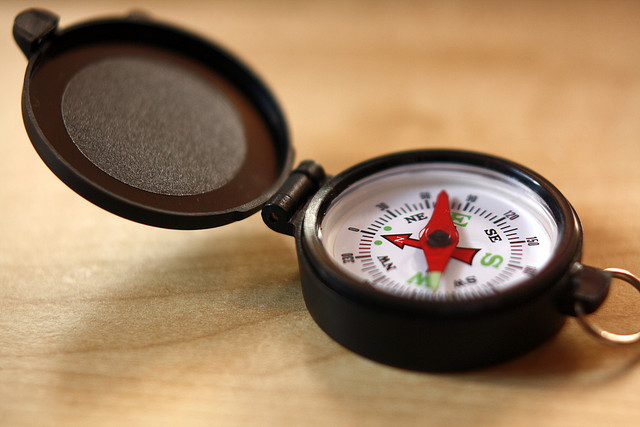
\includegraphics[width=.8\textwidth]{photos/Colin_ZHU.jpg}\par
\textit{ 'n Foto deur Colin Zhu}
\end{center}
\end{minipage}
            

\subsection*{Die Aarde se magneetveld}
            \nopagebreak
In die beeld hieronder kan jy 'n voorstelling van die Aarde se magneetveld sien, wat soortgelyk is aan di\'e van 'n reuse staafmagneet, soos aangedui aan die regterkant van die beeld. Die Aarde het twee geografiese pole wat punte op die Aarde se oppervlak is waar die rotasieas van die Aarde die oppervlak ontmoet. Om dit te visualiseer kan jy enige ronde vrug (soos 'n lemoen) vat en 'n potlood deur  die middel druk sodat dit aan die kant uitkom. As jy die potlood draai, draai die vrug ook en dus is die potlood die rotasie-as en die geografiese pole is waar die potlood die vrug binnegaan en verlaat.


Die Aarde het 'n magneetveld en dus noordelike en suidelike \textbf{magnetiese} pole. As jy die Aarde se magneetveld noukeurig meet sal jy sien dat die magnetiese pole nie op dieselfde plekke is as die geografiese pole nie.

Die Aarde het dus twee stelle noord- en suidpole: \texbf{geografiese pole} en \textbf{magnetiese pole}. \par

\begin{figure}[H] % horizontal\label{m37830*id128275}
\begin{center}
\scalebox{0.95} % Change this value to rescale the drawing.
{
\begin{pspicture}(0,-3.7089062)(15.38,3.72)
\definecolor{color875}{rgb}{0.4,0.4,0.4}
\rput(4.08,3.59){11.5$^{o}$}
\rput(6.0,3.08){Geografiese noord pool}
\rput(1.85,3.30){\color{color875}Magnetiese noord pool}
\psbezier[linewidth=0.04,linecolor=color875,arrowsize=0.05291667cm 2.0,arrowlength=1.4,arrowinset=0.4]{->}(3.74,-1.38)(3.9,-2.10)(4.34,-2.58)(4.98,-2.90)
\psbezier[linewidth=0.04,linecolor=color875,arrowsize=0.05291667cm 2.0,arrowlength=1.4,arrowinset=0.4]{->}(3.58,-1.34)(3.1,-3.26)(1.14,-3.10)(1.02,-3.12)
\psbezier[linewidth=0.04,linecolor=color875,arrowsize=0.05291667cm 2.0,arrowlength=1.4,arrowinset=0.4]{->}(3.54,-1.40)(3.38,-2.12)(2.94,-2.60)(2.3,-2.92)
\psbezier[linewidth=0.04,linecolor=color875,arrowsize=0.05291667cm 2.0,arrowlength=1.4,arrowinset=0.4]{->}(3.54,-1.36)(2.26,-3.04)(0.6,-2.50)(0.48,-2.20)
\psbezier[linewidth=0.04,linecolor=color875,arrowsize=0.05291667cm 2.0,arrowlength=1.4,arrowinset=0.4]{->}(3.52,-1.38)(3.06,-1.96)(2.68,-2.20)(2.06,-2.46)
\psbezier[linewidth=0.04,linecolor=color875,arrowsize=0.05291667cm 3.0,arrowlength=1.4,arrowinset=0.4]{->}(3.41,-1.38)(2.05,-1.72)(1.63,-0.90)(1.59,-0.10)
\psline[linewidth=0.04cm,linecolor=color875,linestyle=dashed,dash=0.16cm 0.16cm](3.62,3.35)(3.62,-3.68)
\psline[linewidth=0.04cm](4.18,3.34)(3.11,-3.48)
\psbezier[linewidth=0.04,linecolor=color875](3.82,1.15)(5.93,2.29)(6.54,-2.14)(3.87,-1.36)
\psbezier[linewidth=0.04,linecolor=color875,arrowsize=0.05291667cm 3.0,arrowlength=1.4,arrowinset=0.4]{->}(3.90,-1.36)(5.20,-1.70)(5.61,-0.88)(5.64,-0.08)
\psbezier[linewidth=0.04,linecolor=color875](3.5,1.13)(1.29,2.27)(0.66,-2.16)(3.44,-1.38)
\psbezier[linewidth=0.04,linecolor=color875](3.7,1.15)(6.84,3.47)(7.28,-3.24)(3.76,-1.36)
\psbezier[linewidth=0.04,linecolor=color875,arrowsize=0.05291667cm 3.0,arrowlength=1.4,arrowinset=0.4]{->}(3.78,-1.38)(5.04,-2.06)(6.1,-1.64)(6.24,-0.068)
\psbezier[linewidth=0.04,linecolor=color875](3.58,1.15)(0.44,3.47)(0.0,-3.24)(3.52,-1.36)
\psbezier[linewidth=0.04,linecolor=color875,arrowsize=0.05291667cm 3.0,arrowlength=1.4,arrowinset=0.4]{->}(3.48,-1.38)(2.22,-2.06)(1.18,-1.64)(1.04,-0.048)
\psbezier[linewidth=0.04,linecolor=color875,arrowsize=0.05291667cm 2.0,arrowlength=1.4,arrowinset=0.4]{<-}(3.68,1.15)(4.16,3.07)(6.12,2.91)(6.24,2.93)
\psbezier[linewidth=0.04,linecolor=color875,arrowsize=0.05291667cm 2.0,arrowlength=1.4,arrowinset=0.4]{<-}(3.58,1.15)(3.1,3.07)(1.14,2.91)(1.02,2.93)
\psbezier[linewidth=0.04,linecolor=color875,arrowsize=0.05291667cm 2.0,arrowlength=1.4,arrowinset=0.4]{->}(3.72,-1.34)(4.2,-3.26)(6.16,-3.10)(6.28,-3.12)
\psbezier[linewidth=0.04,linecolor=color875,arrowsize=0.05291667cm 2.0,arrowlength=1.4,arrowinset=0.4]{<-}(3.76,1.15)(5.0332885,2.83)(6.7,2.29)(6.82,1.99)
\psbezier[linewidth=0.04,linecolor=color875,arrowsize=0.05291667cm 2.0,arrowlength=1.4,arrowinset=0.4]{<-}(3.56,1.15)(2.28,2.83)(0.62,2.29)(0.5,1.99)
\psbezier[linewidth=0.04,linecolor=color875,arrowsize=0.05291667cm 2.0,arrowlength=1.4,arrowinset=0.4]{->}(3.76,-1.36)(5.03,-3.04)(6.7,-2.50)(6.82,-2.20)
\psbezier[linewidth=0.04,linecolor=color875,arrowsize=0.05291667cm 2.0,arrowlength=1.4,arrowinset=0.4]{->}(6.84,2.01)(6.24,2.57)(5.053,2.23)(4.78,2.05)
\psbezier[linewidth=0.04,linecolor=color875,arrowsize=0.05291667cm 2.0,arrowlength=1.4,arrowinset=0.4]{->}(0.48,2.01)(1.08,2.57)(2.26,2.23)(2.54,2.05)
\psbezier[linewidth=0.04,linecolor=color875,arrowsize=0.05291667cm 2.0,arrowlength=1.4,arrowinset=0.4]{->}(6.24,2.93)(5.5,2.95)(4.94,2.75)(4.5,2.45)
\psbezier[linewidth=0.04,linecolor=color875,arrowsize=0.05291667cm 2.0,arrowlength=1.4,arrowinset=0.4]{->}(1.14,2.93)(1.56,2.91)(2.32,2.79)(2.8,2.43)
\psbezier[linewidth=0.04,linecolor=color875,arrowsize=0.05291667cm 2.0,arrowlength=1.4,arrowinset=0.4]{->}(3.78,-1.38)(4.24,-1.96)(4.62,-2.20)(5.24,-2.46)
\rput{-19.00}(0.23,1.16){\pscircle[linewidth=0.04,dimen=outer,fillstyle=solid](3.60,-0.11){1.29}}
\psbezier[linewidth=0.04](3.98,0.27)(3.97,0.31)(3.97,0.31)(3.97,0.32)(3.98,0.33)(3.96,0.37)(3.97,0.36)(3.98,0.35)(3.97,0.34)(3.96,0.34)(3.96,0.35)(4.01,0.36)(3.98,0.36)(3.95,0.36)(3.98,0.47)(3.72,0.45)(3.47,0.43)(3.68,0.56)(3.60,0.57)(3.51,0.58)(3.50,0.57)(3.35,0.55)(3.21,0.53)(3.09,0.52)(2.96,0.37)(2.832,0.2295)(2.731,-0.0794)(2.908,-0.1861)(3.084,-0.292)(3.310,-0.261)(3.358,-0.343)(3.406,-0.426)(3.290,-0.703)(3.383,-0.809)(3.477,-0.914)(3.425,-1.007)(3.469,-1.053)(3.513,-1.099)(3.676,-1.124)(3.738,-1.066)(3.801,-1.008)(3.855,-0.837)(3.958,-0.8094)(4.0619,-0.7816)(4.004,-0.485)(4.127,-0.434)(4.249,-0.383)(4.382,-0.238)(4.426,-0.166)(4.469,-0.0952)(4.290,-0.185)(4.173,-0.1098)(4.055,-0.0342)(3.994,0.232)(3.983,0.274)
\psbezier[linewidth=0.04](3.940,0.38)(3.92,0.18)(4.33,-0.04)(4.28,-0.045)(4.24,-0.046)(4.55,0.012)(4.52,0.17)(4.49,0.33)(4.18,0.074)(4.27,0.27)(4.36,0.47)(4.88,-0.05)(4.81,0.03)(4.74,0.11)(4.8,0.41)(4.6,0.56)(4.51,0.71)(4.24,1.14)(3.85,1.09)(3.47,1.04)(3.89,0.82)(3.58,0.93)(3.27,1.04)(3.07,0.58)(3.28,0.65)(3.48,0.72)(3.72,0.68)(3.76,0.65)(3.80,0.63)(3.95,0.54)(4.08,0.61)(4.20,0.68)(4.15,0.00)(3.97,0.30)
\psbezier[linewidth=0.04](2.35,0.13)(2.53,-0.64)(2.64,-0.19)(2.68,-0.45)(2.72,-0.71)(2.67,-0.57)(2.69,-0.81)(2.71,-1.05)(2.73,-1.08)(2.72,-0.99)(2.71,-0.91)(2.63,-1.11)(2.70,-0.99)
\psarc[linewidth=0.04](3.86,2.91){0.34}{37.87}{135.0}

\psbezier[linewidth=0.04,linecolor=color875,arrowsize=0.05291667cm 2.0,arrowlength=1.4,arrowinset=0.4]{->}(11.82,-1.36)(11.98,-2.08)(12.42,-2.56)(13.06,-2.88)
\psbezier[linewidth=0.04,linecolor=color875,arrowsize=0.05291667cm 2.0,arrowlength=1.4,arrowinset=0.4]{->}(11.66,-1.32)(11.18,-3.24)(9.22,-3.0)(9.1,-3.10)
\psbezier[linewidth=0.04,linecolor=color875,arrowsize=0.05291667cm 2.0,arrowlength=1.4,arrowinset=0.4]{->}(11.62,-1.38)(11.46,-2.10)(11.02,-2.58)(10.38,-2.90)
\psbezier[linewidth=0.04,linecolor=color875,arrowsize=0.05291667cm 2.0,arrowlength=1.4,arrowinset=0.4]{->}(11.62,-1.34)(10.34,-3.02)(8.68,-2.48)(8.56,-2.18)
\psbezier[linewidth=0.04,linecolor=color875,arrowsize=0.05291667cm 2.0,arrowlength=1.4,arrowinset=0.4]{->}(11.6,-1.36)(11.14,-1.94)(10.76,-2.18)(10.14,-2.44)
\psbezier[linewidth=0.04,linecolor=color875,arrowsize=0.05291667cm 3.0,arrowlength=1.4,arrowinset=0.4]{->}(11.49,-1.36)(10.13,-1.70)(9.71,-0.88)(9.67,-0.08)
\psline[linewidth=0.04cm,linecolor=color875,linestyle=dashed,dash=0.16cm 0.16cm](11.7,3.3710938)(11.7,-3.6689062)
\psbezier[linewidth=0.04,linecolor=color875](11.9,1.17)(14.01,2.31)(14.62,-2.12)(11.9,-1.34)
\psbezier[linewidth=0.04,linecolor=color875,arrowsize=0.05291667cm 3.0,arrowlength=1.4,arrowinset=0.4]{->}(11.98,-1.34)(13.28,-1.68)(13.69,-0.86)(13.72,-0.06)
\psbezier[linewidth=0.04,linecolor=color875](11.58,1.15)(9.37,2.29)(8.74,-2.14)(11.52,-1.36)
\psbezier[linewidth=0.04,linecolor=color875](11.78,1.17)(14.92,3.49)(15.36,-3.22)(11.84,-1.34)
\psbezier[linewidth=0.04,linecolor=color875,arrowsize=0.05291667cm 3.0,arrowlength=1.4,arrowinset=0.4]{->}(11.86,-1.36)(13.12,-2.04)(14.18,-1.62)(14.32,-0.04)
\psbezier[linewidth=0.04,linecolor=color875](11.66,1.17)(8.52,3.49)(8.08,-3.22)(11.6,-1.34)
\psbezier[linewidth=0.04,linecolor=color875,arrowsize=0.05291667cm 3.0,arrowlength=1.4,arrowinset=0.4]{->}(11.56,-1.36)(10.3,-2.04)(9.26,-1.62)(9.12,-0.02)
\psbezier[linewidth=0.04,linecolor=color875,arrowsize=0.05291667cm 2.0,arrowlength=1.4,arrowinset=0.4]{<-}(11.76,1.17)(12.24,3.09)(14.2,2.93)(14.32,2.95)
\psbezier[linewidth=0.04,linecolor=color875,arrowsize=0.05291667cm 2.0,arrowlength=1.4,arrowinset=0.4]{<-}(11.66,1.17)(11.18,3.09)(9.22,2.93)(9.1,2.95)
\psbezier[linewidth=0.04,linecolor=color875,arrowsize=0.05291667cm 2.0,arrowlength=1.4,arrowinset=0.4]{->}(11.8,-1.32)(12.28,-3.24)(14.24,-3.08)(14.36,-3.10)
\psbezier[linewidth=0.04,linecolor=color875,arrowsize=0.05291667cm 2.0,arrowlength=1.4,arrowinset=0.4]{<-}(11.84,1.17)(13.11,2.85)(14.78,2.31)(14.9,2.01)
\psbezier[linewidth=0.04,linecolor=color875,arrowsize=0.05291667cm 2.0,arrowlength=1.4,arrowinset=0.4]{<-}(11.64,1.17)(10.36,2.85)(8.7,2.31)(8.58,2.01)
\psbezier[linewidth=0.04,linecolor=color875,arrowsize=0.05291667cm 2.0,arrowlength=1.4,arrowinset=0.4]{->}(11.84,-1.34)(13.11,-3.02)(14.78,-2.48)(14.9,-2.18)
\psbezier[linewidth=0.04,linecolor=color875,arrowsize=0.05291667cm 2.0,arrowlength=1.4,arrowinset=0.4]{->}(14.92,2.03)(14.32,2.59)(13.13,2.25)(12.86,2.07)
\psbezier[linewidth=0.04,linecolor=color875,arrowsize=0.05291667cm 2.0,arrowlength=1.4,arrowinset=0.4]{->}(8.56,2.03)(9.16,2.59)(10.34,2.25)(10.62,2.07)
\psbezier[linewidth=0.04,linecolor=color875,arrowsize=0.05291667cm 2.0,arrowlength=1.4,arrowinset=0.4]{->}(14.32,2.95)(13.58,2.97)(13.02,2.77)(12.58,2.47)
\psbezier[linewidth=0.04,linecolor=color875,arrowsize=0.05291667cm 2.0,arrowlength=1.4,arrowinset=0.4]{->}(9.22,2.95)(9.64,2.93)(10.4,2.81)(10.88,2.45)
\psbezier[linewidth=0.04,linecolor=color875,arrowsize=0.05291667cm 2.0,arrowlength=1.4,arrowinset=0.4]{->}(11.86,-1.36)(12.32,-1.94)(12.7,-2.18)(13.32,-2.44)
\psframe[fillstyle=solid,fillcolor=red,linewidth=0.04,dimen=outer,fillstyle=solid](12.2,1.23)(11.22,-1.36)
\rput(11.65,0.96){S}
\rput(11.72,-1.09){N}
\end{pspicture} 
}\end{center}
 \end{figure}       
        \par 
Daar word gemeen dat die Aarde se magneetveld deur vloeiende gesmelte metale in die buitenste kern van die Aarde veroorsaak word. Die vloeiende metaal veroorsaak elektriese strome en dus magneetvelde. In die diagram kan jy sien dat die rigting van magnetiese noord en ware noord nie identies is nie. Die \textbf{geografiese noord pool}, wat die punt is waardeur die rotasie as gaan, is omtrent 11,5$^{\circ}$ weg van die rigting van die \textbf{magnetiese noord pool} (wat die punt is waarna die kompas sal wys). Die magnetiese pole skuif effens rond met tyd. \par
\IFact{Die Aarde se magnetiese pole ruil posisies om elke 200~000 jaar!. Jy kan dit sien as 'n staafmagneet wat se noord- en suidpole periodies kante ruil. Die rede hiervoor word nog nie goed verstaan nie}

Nog 'n interessante ding om te weet is dat as ons dink aan die Aarde as 'n reuse staafmagneet, en ons weet dat die magnetiese veldlyne altyd van \textsl{noord na suid} wys, dat dit wat ons die \textsl{magnetiese noordpool} noem eintlik die \textsl{suidpool} van 'n staafmagneet is.



\subsection{Verskynsels verwant aan die Aarde se magneetveld}
            \nopagebreak
\label{m37830*fs-id7505799}

\subsection{Die belangrikheid van die magneetveld vir lewe op Aarde}
            \nopagebreak

Die Aarde se magneetveld is baie belangrik vir mense en ander diere want dit beskerm ons van ho\"e energie gelaaide deeltjies wat deur die son vrygelaat word. Die stroom van gelaaide deeltjies (meestal protone en elektrone) wat afkomstig is van die son word die sonwind genoem. Wanneer hierdie deeltjies naby aan die Aarde kom word hulle vasgevang in die magneetveld en kan dus nie neerre\"en op die oppervlak waar hulle kan skade doen aan lewende organismes nie. Ruimtevaarders loop ook die risiko om deur die sonwind bestraal te word omdat hulle nie altyd in die gebiede is waar die magneetveld hulle sal beskerm nie.\par

\label{m37830*fs-id1166236522828}
\begin{minipage}{.5\textwidth}
 \begin{center}
  \textbf{Grafiese tentoonstelling van die magnetosfeer}\par
  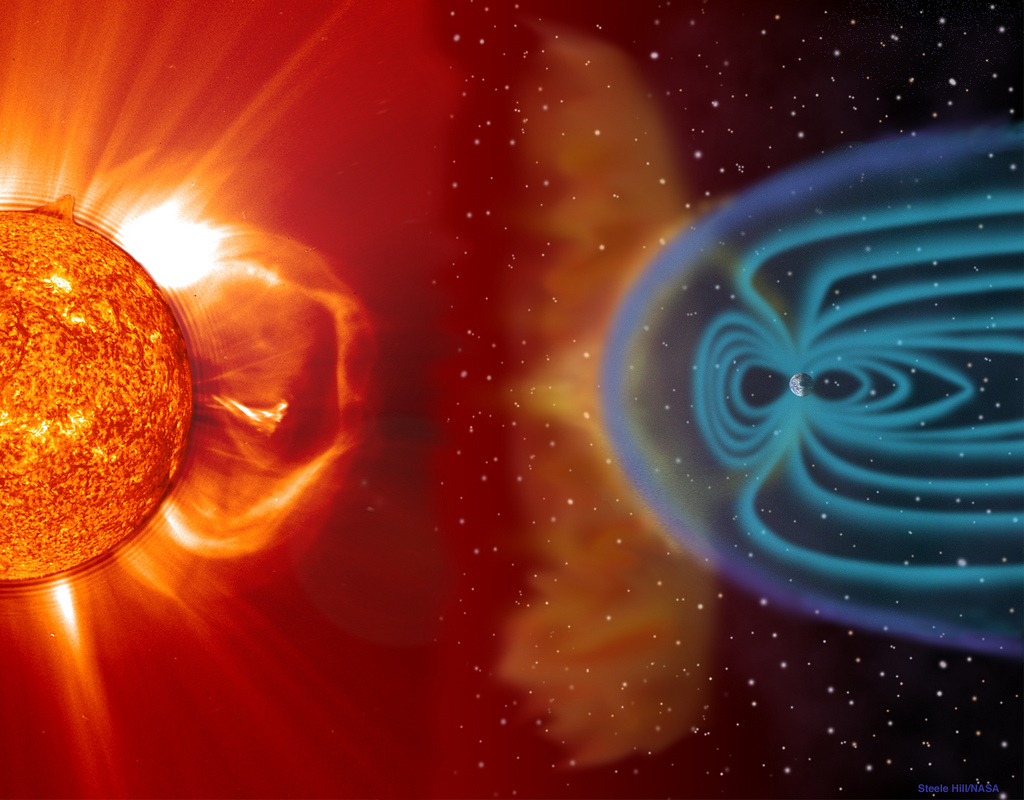
\includegraphics[width=.8\textwidth]{photos/magnetosphere.jpg}\par
  \textit{Grafika deur NASA Goddard Foto en Video op Flickr}
 \end{center}
\end{minipage}
\begin{minipage}{.5\textwidth}

Die area bo die Aarde se atmosfeer waarin die gelaaide deeltjies geaffekteer word deur die Aarde se magneetveld word die magnetosfeer genoem. Redelik gereeld, bykomend tot die sonwind, mag daar 'n groot bondel deeltjies met hul eie magneetveld afkomstig van die son uitgeskiet word. Soms beweeg hierdie bondels na die Aarde waar hulle magneetvelde kan meng met di\'e van die Aarde. Wanneer dit gebeur word daar 'n groot hoeveelheid energie vrygelaat in die Aarde se magnetosfeer en veroorsaak 'n geomagnetiese storm. Hierdie storms veroorsaak skielike veranderings in die Aarde se magnetosfeer wat elektriese en magnetiese stelses soos krag- en selfoonnetwerke kan be\"invloed.

\end{minipage}
\par 


\subsection{Poolligte}
\nopagebreak
\label{m37830*fs-id1166211416999}

 'n Ander effek wat deur die magneetveld veroorsaak word is die skouspelagtige noordpoollig (noorderlig) en suidpoollig (suiderlig), wat ook die ``Aurora Borealis'' en ``Aurora Australis'' genoem word. \par

\begin{minipage}{.6\textwidth}
Wanneer gelaaide deeltjies van die sonwind die Aarde se magneetveld bereik, volg hulle 'n spiraalpad op die magnetiese veldlyne na die noord en suid pole toe. As hulle bots met deeltjies in die Aarde se atmosfeer veroorsaak hulle die rooi en groen lig wat oor 'n groot deel van die lug strek wat die ``aurora'' genoem word.
\begin{center}
  \textbf{Aurora borealis gefotografeer in Alaska}\par
  \includegraphics[width=.8\textwidth]{photos/aurora_borealis_Trodel.jpg}\par
  \textit{Foto deur Trodel op Flickr}
 \end{center}
\end{minipage}
\begin{minipage}{.4\textwidth}
 \begin{center}
  \textbf{Aurora australis gefotografeer vanuit die ruimte}\par
  \includegraphics[width=.9\textwidth]{photos/aurora_australis_seishin17.jpg}\par
  \textit{Foto deur seishin17 op Flickr}
 \end{center}
\end{minipage}


Aangesien dit net naby die Noord en Suid pole gebeur, kan ons nie aurora sien in Suid-Afrika nie, alhoewel mense wat by ho\"e breedtegrade bly in Kanada, Swede en Finland, byvoorbeeld, gereeld die noorderlig sien.
\par 




\summary{VPfjh}
            \nopagebreak
\begin{itemize}[noitemsep ] 
\item Magnete het twee pole - Noord en Suid
\item Sommige stowwe kan maklik magneties gemaak word
\item Identiese pole stoot mekaar af en teenoorgestelde pole trek mekaar aan
\item Die Aarde het ook 'n magneetveld
\item 'n Kompas kan gebruik word om die rigting na die magnetiese noordpool te vind en help ons om ons rigting te vind.
\end{itemize}

\begin{eocexercises}
\nopagebreak
\begin{enumerate}[noitemsep, label=\textbf{\arabic*}. ] 
\item Verduidelik wat word bedoel met die term \textsl{magneetveld}
\item Gebruik woorde en sketse om te verduidelik hoekom permanente magnete 'n magneetveld rondom hulle het. Verwys na \textsl{domeine} in jou verduideliking.
\item Wat is 'n magneet?
\item Wat gebeur met die pole van 'n magneet as jy dit in stukke opsny?
\item Wat gebeur as jy soortgelyke magnetiese pole nader aan mekaar bring?
\item Wat gebeur as jy teenoorgestelde magnetiese pole nader aan mekaar bring?
\item Skets die magneetveld wat rondom 'n staafmagneet is.
\item Verduidelik hoe 'n kompas die rigting van 'n magneetveld aanwys.
\item Vergelyk die magneetveld van die Aarde met di\'e van 'n staafmagneet. Maak gebruik van beskrywings en sketse.
\item Verduidelik die verskil tussen die geografiese noordpool en die magnetiese noordpool van die Aarde.
\item Gee twee voorbeelde van verskynsel wat deur die Aarde se magneetveld be\"invloed word. 
\item Maak 'n skets van die Aarde se magneetveld.
\end{enumerate}
\practiceinfo
 \par \begin{tabular}[h]{cccccc}
 (1.) 029h  &  (2.) 029i  &  (3.) 029j  &  (4.) 029k  &  (5.) 029m  &  (6.) 029n  &  (7.) 029p  &  (8.) 029q  &  (9.) 029r  &  (10.) 029s  &  (11.) 029t  &  (12.) 029u  & \end{tabular}
\end{eocexercises}
